\mychapter{Derivades i aplicacions}{Derivades i les seves aplicacions}{
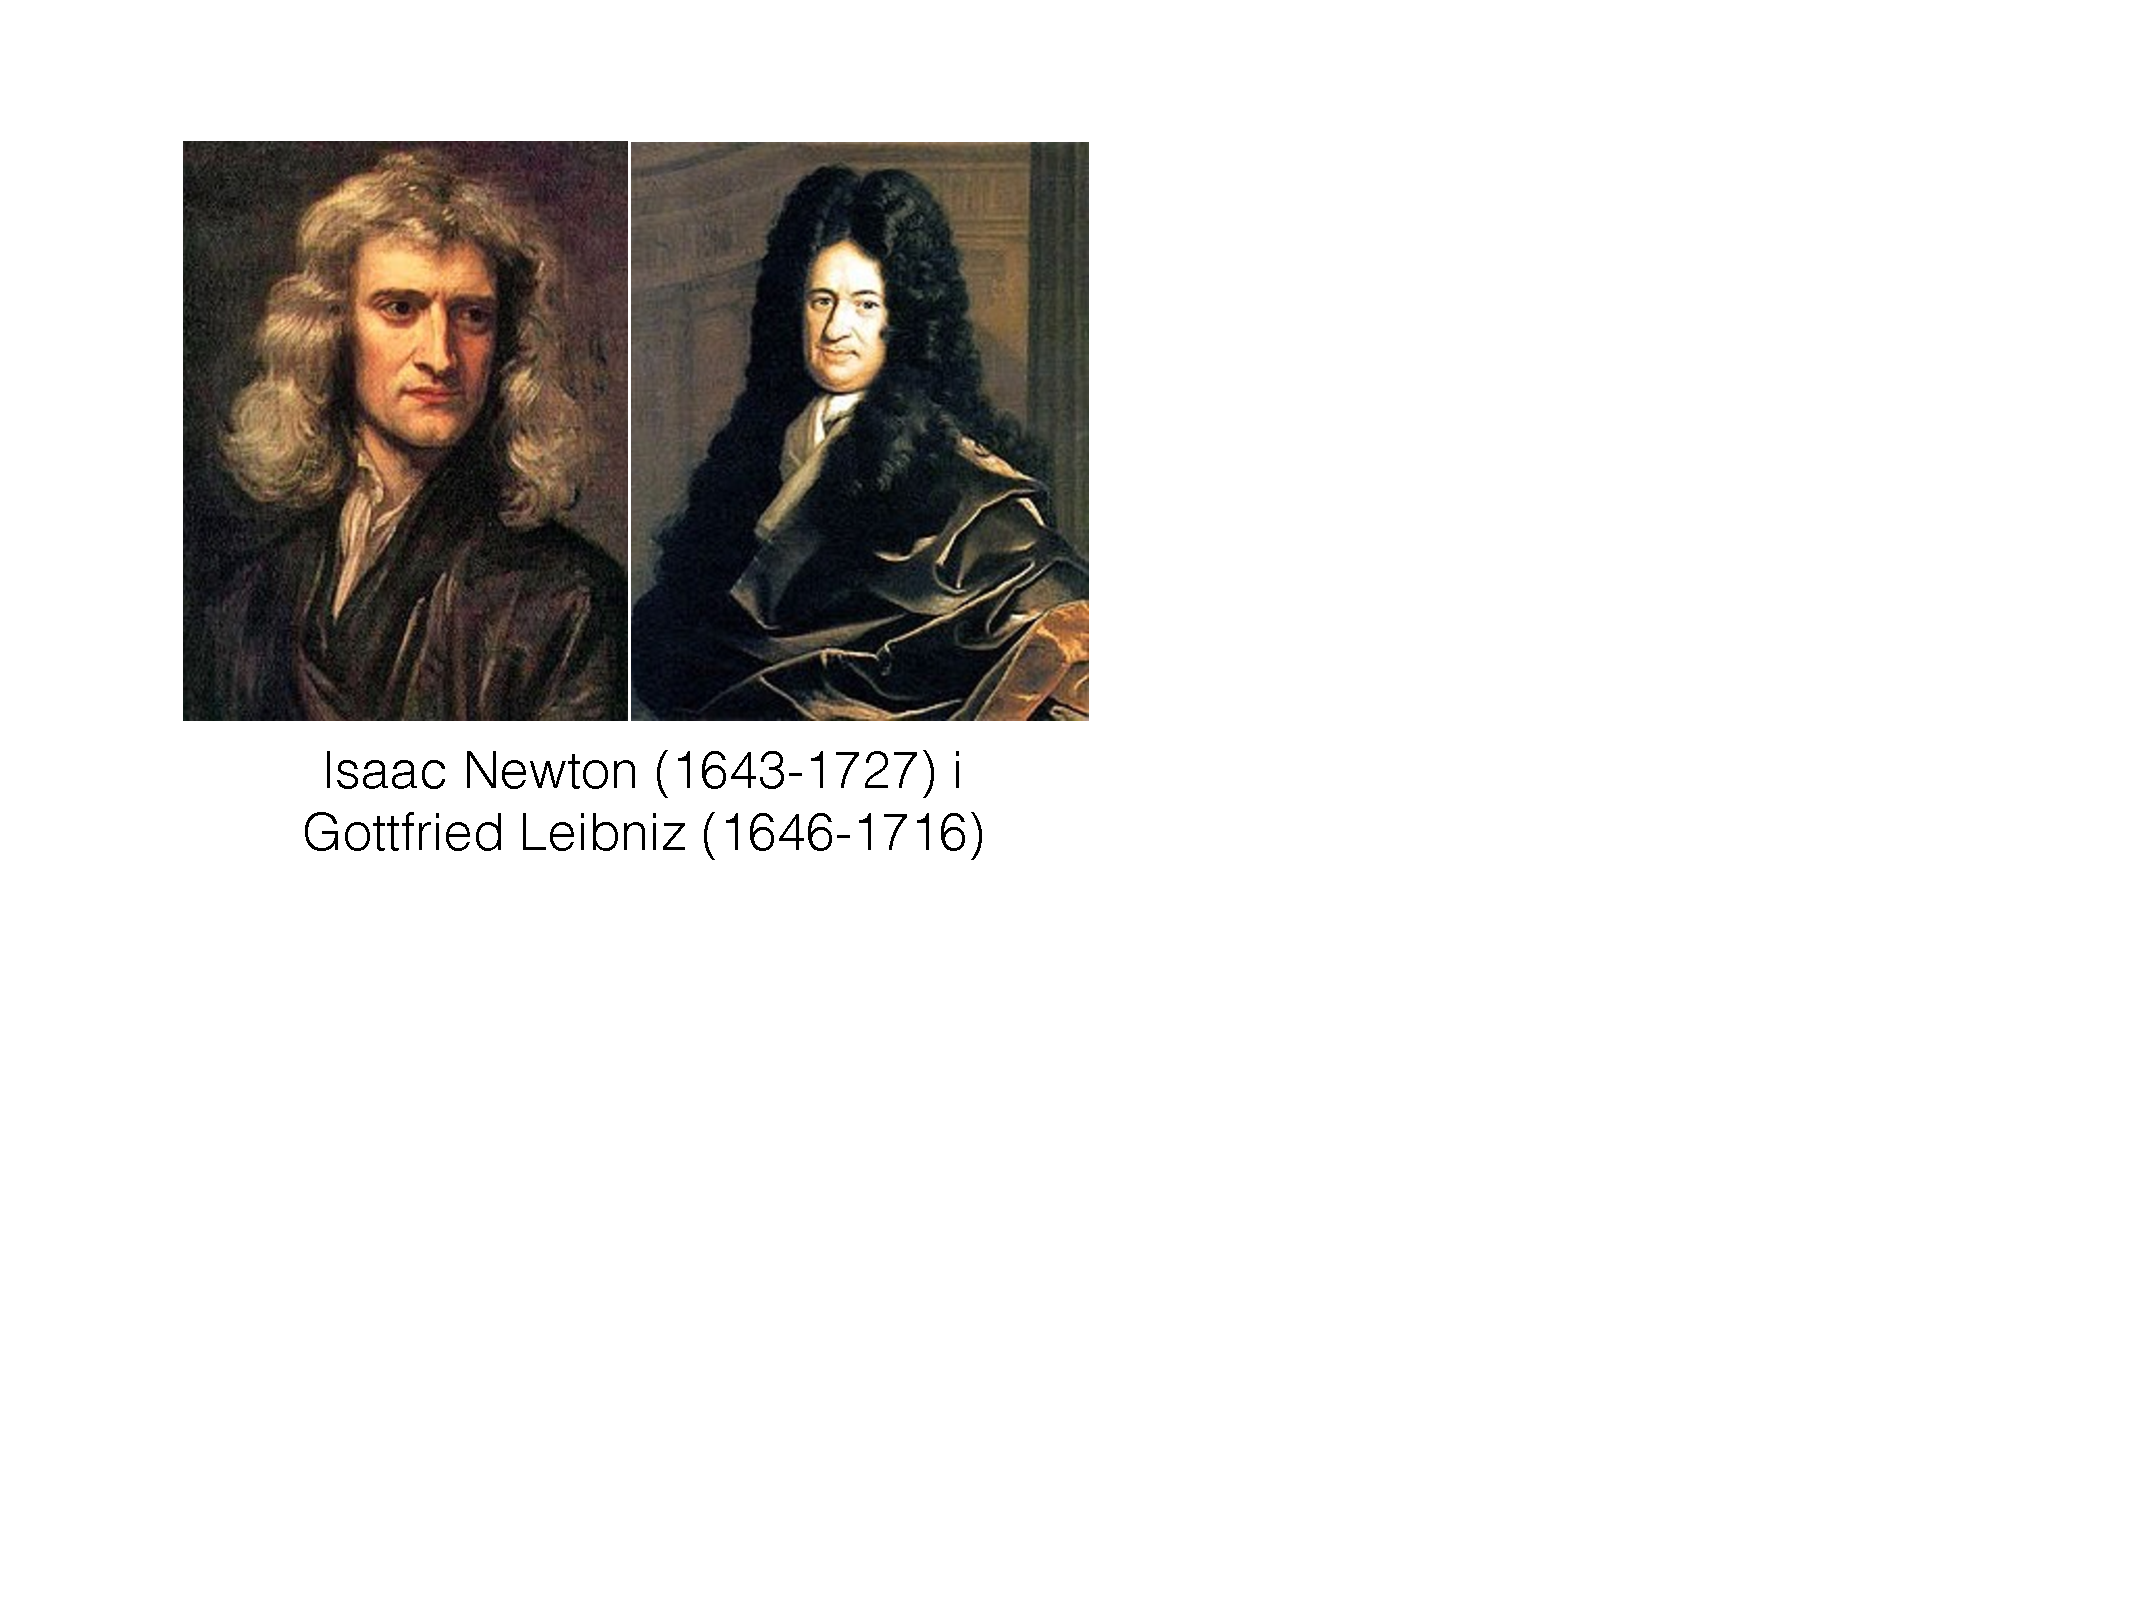
\includegraphics[width=4.5cm]{img-07/chap8.pdf}
}{chap:derivades}

\section{Concepte de derivada}

\begin{theorybox}
	\begin{minipage}{0.6\textwidth}
		La \textbf{taxa de variació mitjana} (TVM) d'una funció en un interval $[a,\, b]$ es defineix com:
		\begin{equation*}
		TVM[a,b] = \frac{f(b)-f(a)}{b-a}
		\end{equation*}
		i correspon al \textbf{pendent de la recta secant} a la funció en els punts d'abscisses $a$ i $b$.
	\end{minipage}
	\begin{minipage}{0.38\textwidth}
		\centering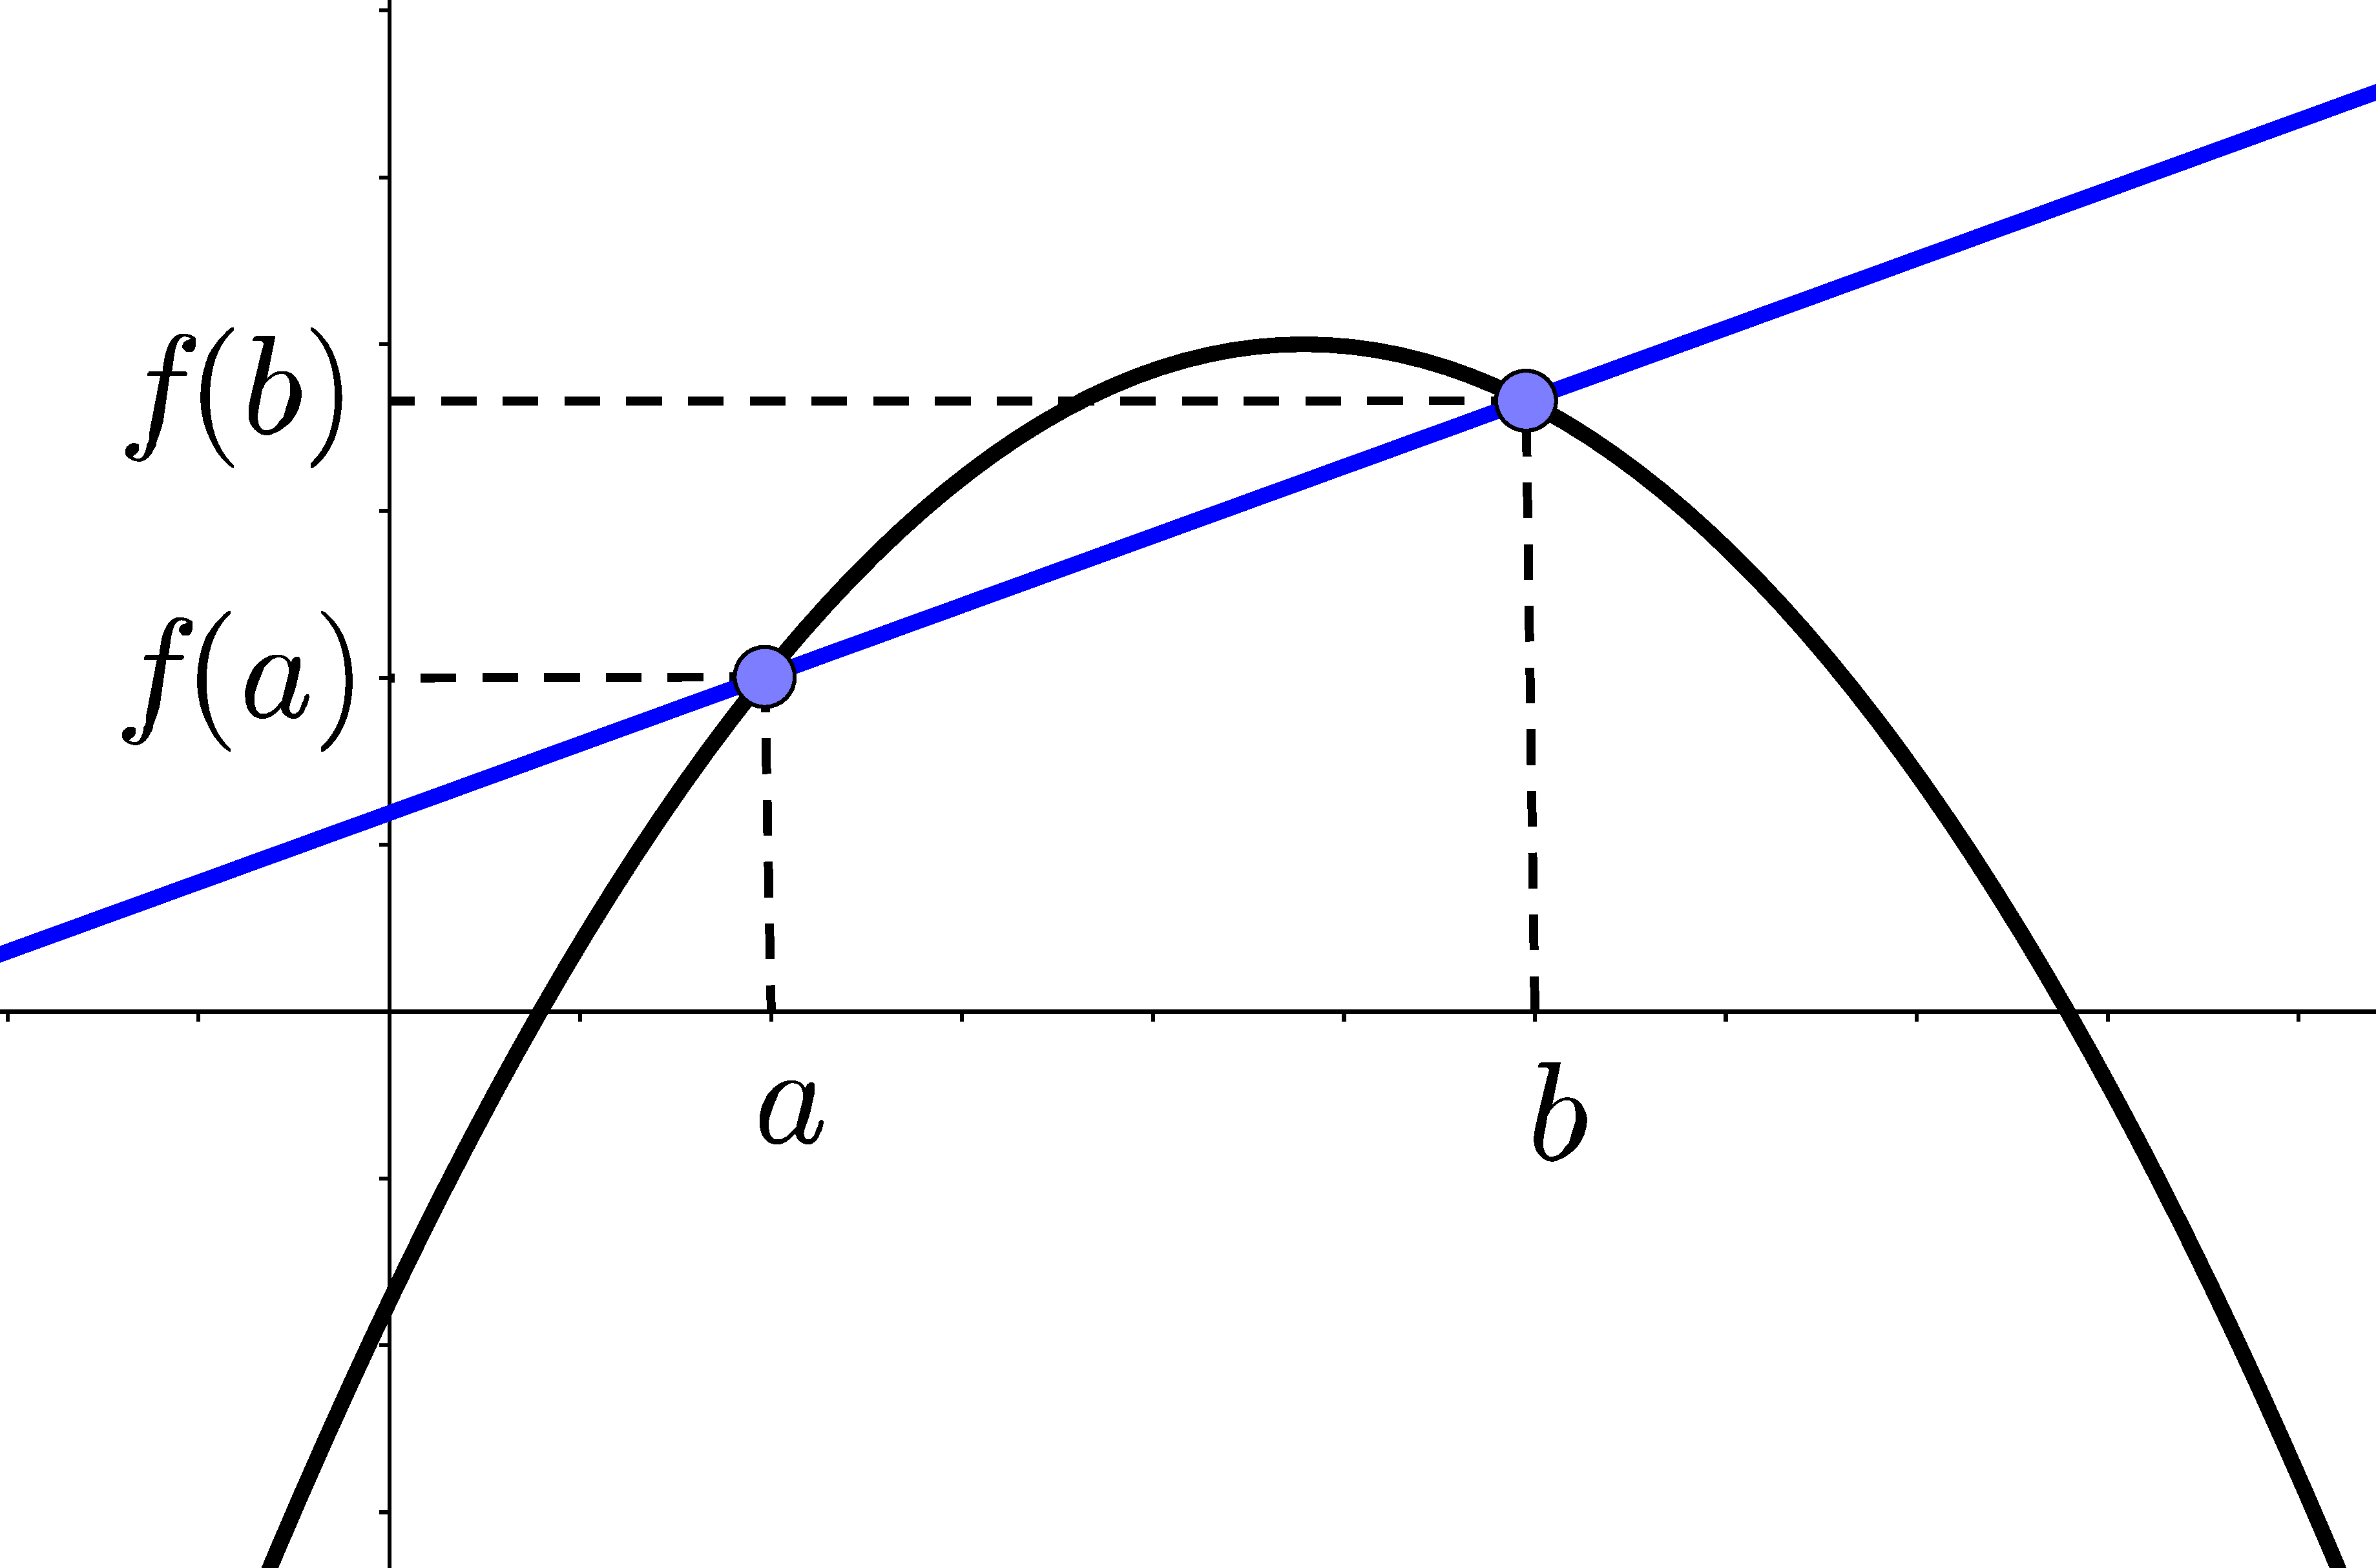
\includegraphics[width=0.9\textwidth]{img-07/rectasecant}
	\end{minipage}
\end{theorybox}

\begin{mylist}
	

\exer Troba la taxa de variació mitjana en els intervals [-3, 2], [1, 5] i [0, 3] de les funcions següents:
\begin{tasks}(4)
\task $y = 3x - 4$   \task $y = -2x - 3$   \task $y = 0.5x + 2$   \task $y = x - 1$ 
\end{tasks}
\noindent A la vista del que has obtingut, creus que la taxa de variació mitjana de les funcions polinòmiques de primer grau és sempre constant i igual al pendent de la recta que la representa?

\answers{[TVM=3, TVM=-2, TVM=0.5, TVM=1]}

\exer  Troba la taxa de variació mitjana de la funció $y = x^2 - 1$ en els intervals [-3, 2], [1, 5] i [0, 3]. És ara constant?

\answers{TVM[-3, 2]=--1, TVM[1, 5]=6 i TVM[0, 3]=3}

\exer  Troba la taxa de variació mitjana de la funció $y= x^3+ 1$ en els intervals [-3, 2], [1, 5] i [0, 3].
Hauràs comprovat que en els dos últims exercicis la taxa de variació mitjana no és constant.

\answers{TVM[-3, 2]=7, TVM[1, 5]=31, TVM[0, 3]=9}

\exer  En fer un estudi sobre l'aterratge d'avions es grava una pel·lícula des del moment en què l'avió toca terra fins que es para, i es mesuren els temps i les distàncies recorregudes:

\begin{tabular}{|p{1.5in}|p{0.3in}|p{0.3in}|p{0.3in}|p{0.3in}|p{0.3in}|p{0.3in}|p{0.3in}|p{0.3in}|} \hline 
	\textbf{Temps ($t$) en segons} & 0 & 2 & 4 & 6 & 8 & 10 & 12 & 14 \\ \hline 
	\textbf{Distància ($d$) en metres} & 0 & 100 & 175 & 230 & 270 & 300 & 325 & 340 \\ \hline 
\end{tabular}

\begin{tasks}
\task Calcula la velocitat mitjana de l'avió. 
\task Calcula la velocitat mitjana en els intervals: [0, 6], [2, 10] i [6, 14].
\task És constant?
\end{tasks}
\answers{[$v_m = 24,3$ m/s, $v_m [0,6] = 38,3$ m/s; $v_m[2,10] = 25$ m/s; $v_m[6,14] = 13,7$ m/s, No és constant. La
 velocitat va disminuint.
 ]}


\exer  S'estudia la posició d'un cotxe respecte de la sortida d'un túnel i s'obtenen les dades següents:

\begin{tabular}{|p{1.2in}|p{0.3in}|p{0.3in}|p{0.3in}|p{0.3in}|p{0.3in}|p{0.3in}|p{0.3in}|p{0.3in}|p{0.3in}|} \hline 
	\textbf{Temps (segons)} & 0 & 5 & 10 & 15 & 20 & 25 & 30 & 35 & 40 \\ \hline 
	\textbf{Distància (metres)} & 0 & 100 & 200 & 290 & 370 & 430 & 510 & 610 & 720 \\ \hline 
\end{tabular}

\begin{tasks}
\task Calcula la velocitat mitjana del cotxe en l'interval [0, 40].
\task Calcula la velocitat mitjana en els intervals [15, 25] i [20, 30]. És constant?
\task Si la velocitat màxima permesa és de 120 km/h, consideres que ha pogut sobrepassar-la en algun moment? I si la velocitat màxima anés de 80 km/h?
\end{tasks}


\answers{[ $v_m [0,40] = 18$ m/s,   $v_m [15,25] = 14$ m/s; $v_m [20,30] = 13$ m/s. No és constant,
	 120 km/h = 33 m/s. Sembla difícil que l'hagi sobrepassat. 80 km/h = 22,2 m/s. No és possible assegurar que no hi hagi anat més
	depresa ja que en el primer interval la seva velocitat mitjana és de 20 m/s.]}

\begin{comment}
\exer  El tren AVE surt de l'estació i augmenta la seva velocitat fins a arribar a 250 km/h en 10 minuts, manté llavors aquesta velocitat constant durant hora i mitja, i comença a disminuir-la fins a parar-se en altres 10 minuts. 

\begin{enumerate}
\exer Representa en una gràfica la funció temps - velocitat.

\exer Ja saps que l'acceleració ens indica la variació de velocitat. Indica l'acceleració mitjana en els primers 10 minuts. 

\exer Indica l'acceleració mitjana entre el minut 10 i el minut 90.

\exer Determina l'acceleració en els últims 10 minuts.
\end{enumerate}
\end{comment}



\begin{comment}	
\exer  En el viatge de l'activitat d'introducció el cotxe recorria entre la primera hora i la segona una distància y donada per l'equació: $y = 0'2x^2 + 110x - 67'2$. Determina la velocitat que portava el cotxe per a  $x = 1'5$. 


	
\exer  En aquest viatge la distància recorreguda per $2'5 \leq x \leq 3$ ve donada per l'equació $y = 110x - 121'4$. I per $3  \leq  x \leq 5$ per  $y = 0'1x^2 + 118x - 146'3$. Per a  $x = 3$ hi ha un canvi en la velocitat.  Calcula la velocitat abans de $x = 3$, i la velocitat després de $x = 3$.
\end{comment}

\end{mylist}

\begin{theorybox}[Derivada en un punt]
	
\video{183}{Definició de derivada}

		La \textbf{derivada d'una funció $f'(a)$} en un punt $x=a$ es defineix com:
	\begin{equation}
	\label{eq:defderiv}
	f'(a)  = \limx[a]{b}\frac{f(b)-f(a)}{b-a} = \limx[h]{0}\frac{f(a+h)-f(a)}{h}
	\end{equation}
	i proporciona el \textbf{pendent de la recta tangent} a la funció en els punt d'abscissa $a$.
	
	\begin{center}
	\begin{minipage}{0.4\textwidth}
		\centering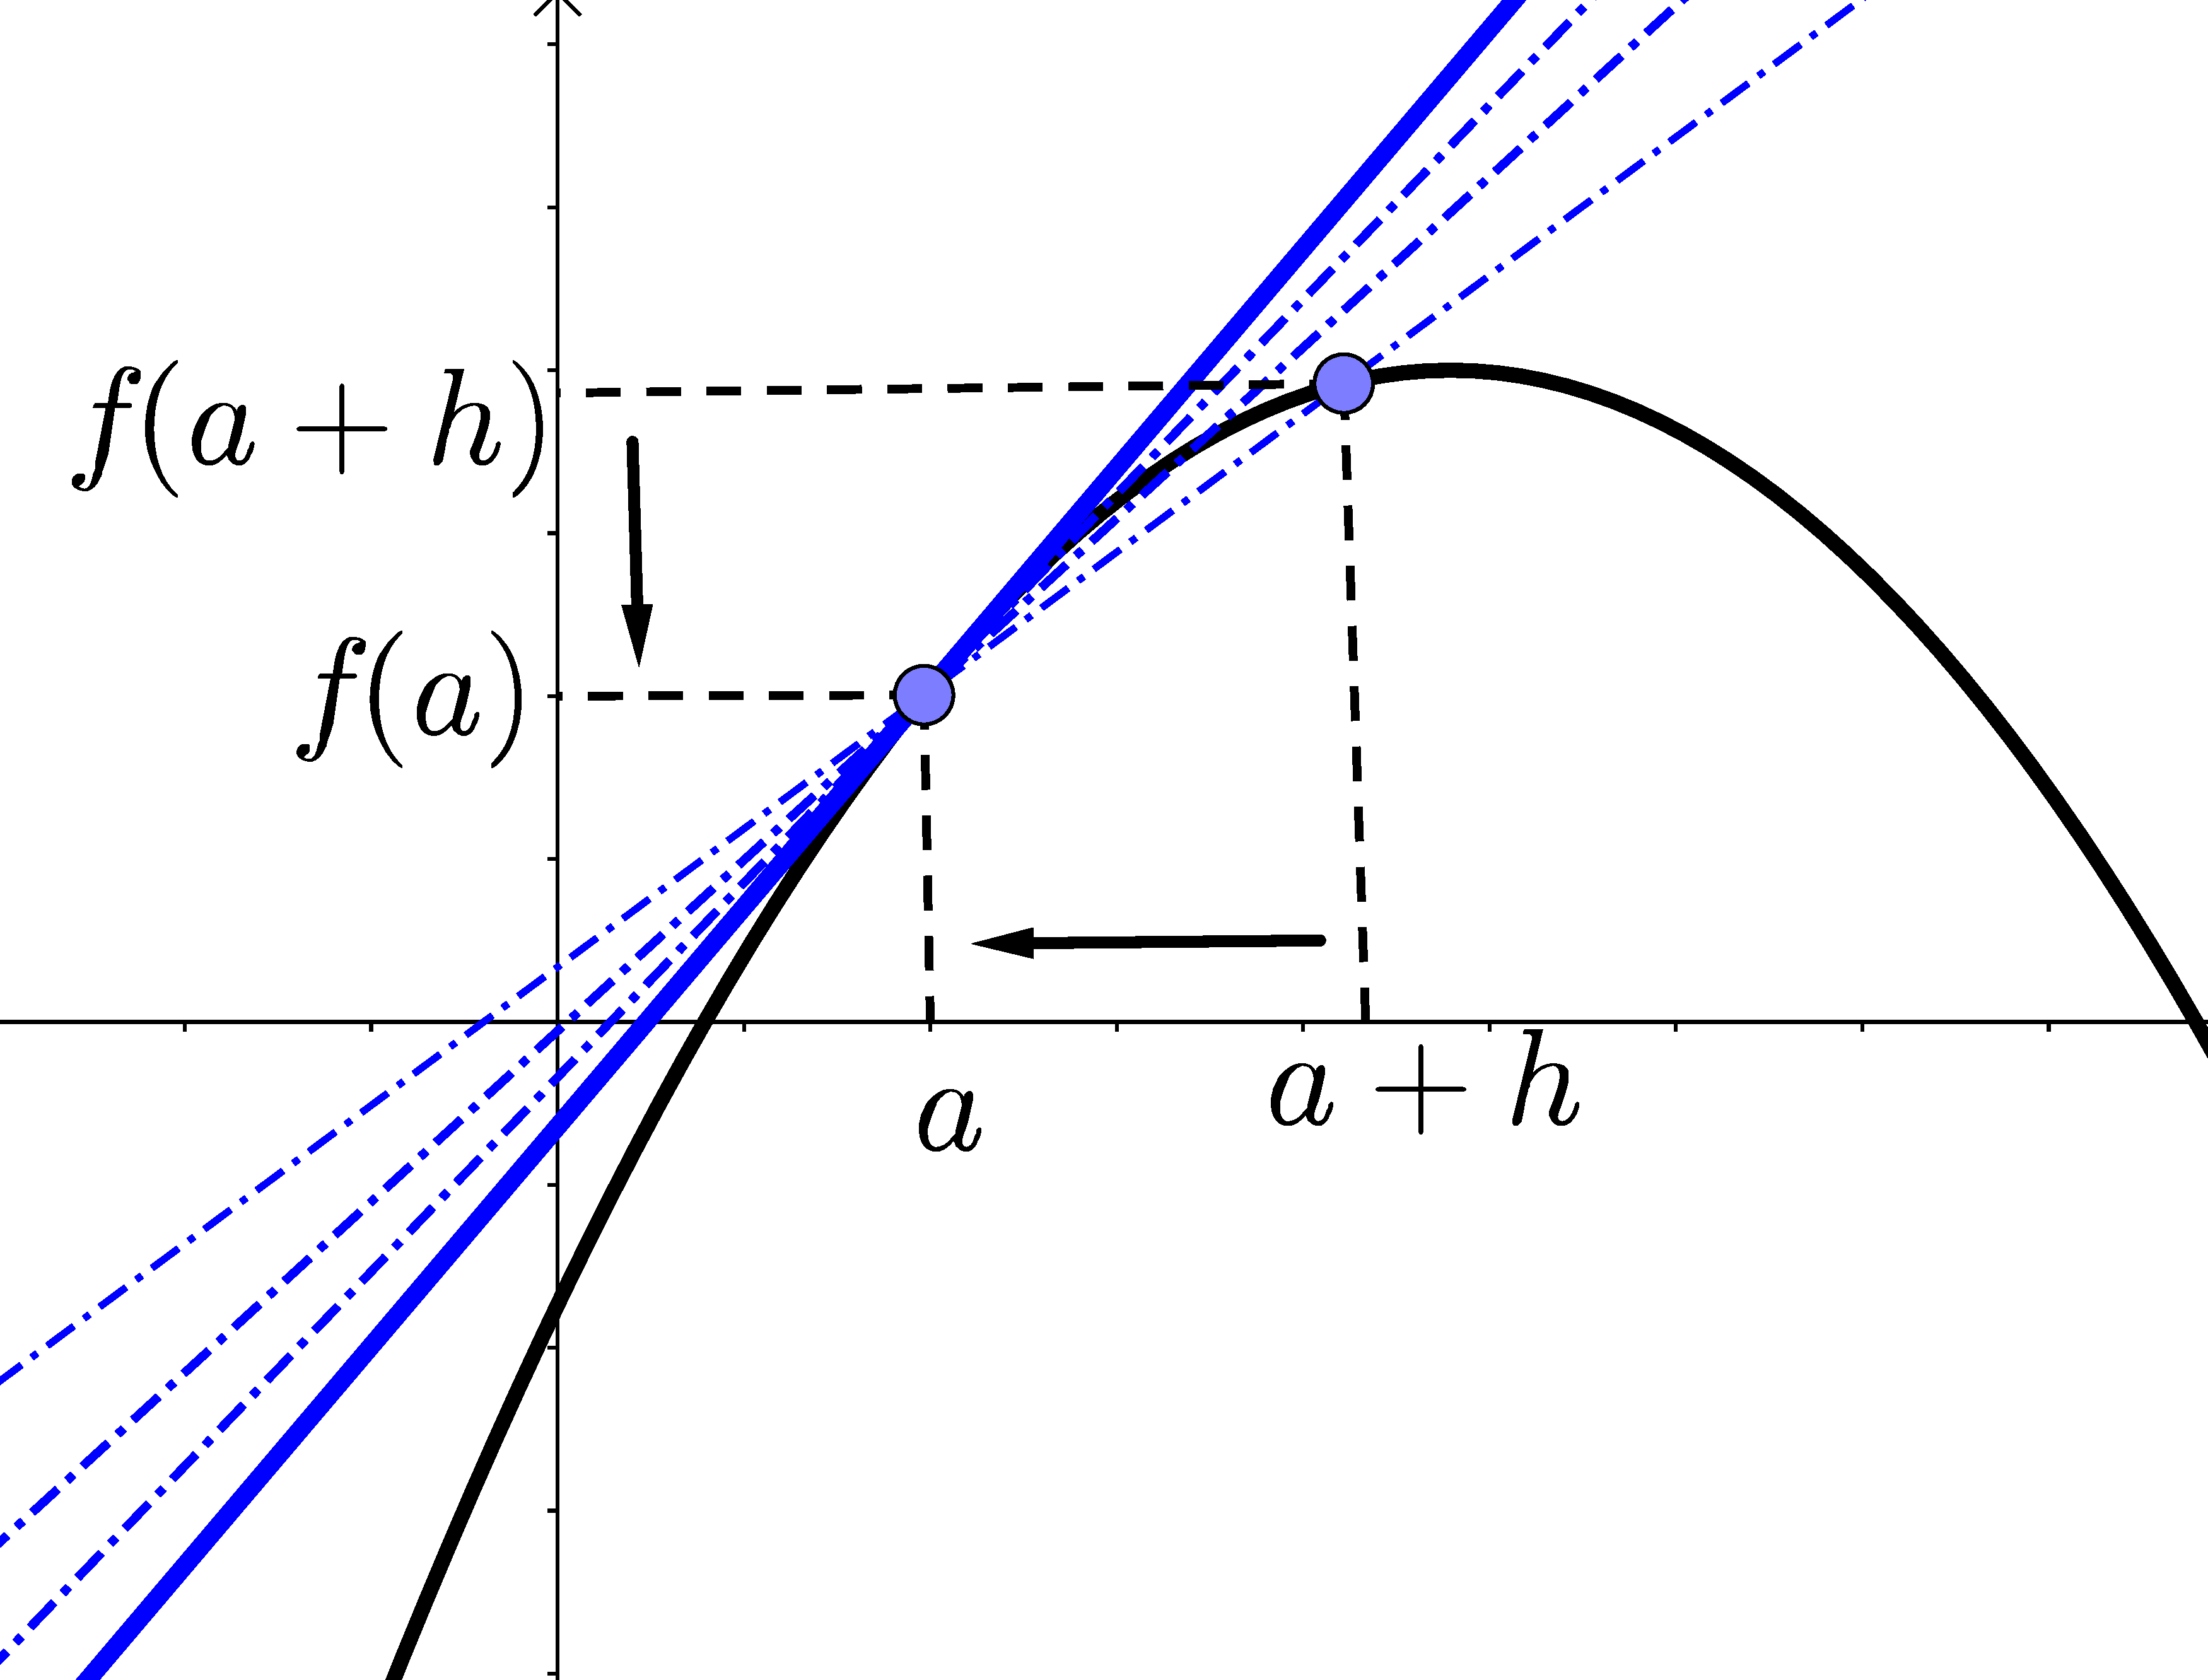
\includegraphics[width=0.9\textwidth]{img-07/rectatangent}
	\end{minipage}
\hspace{0.5cm}
 	\begin{minipage}{0.4\textwidth}
		\centering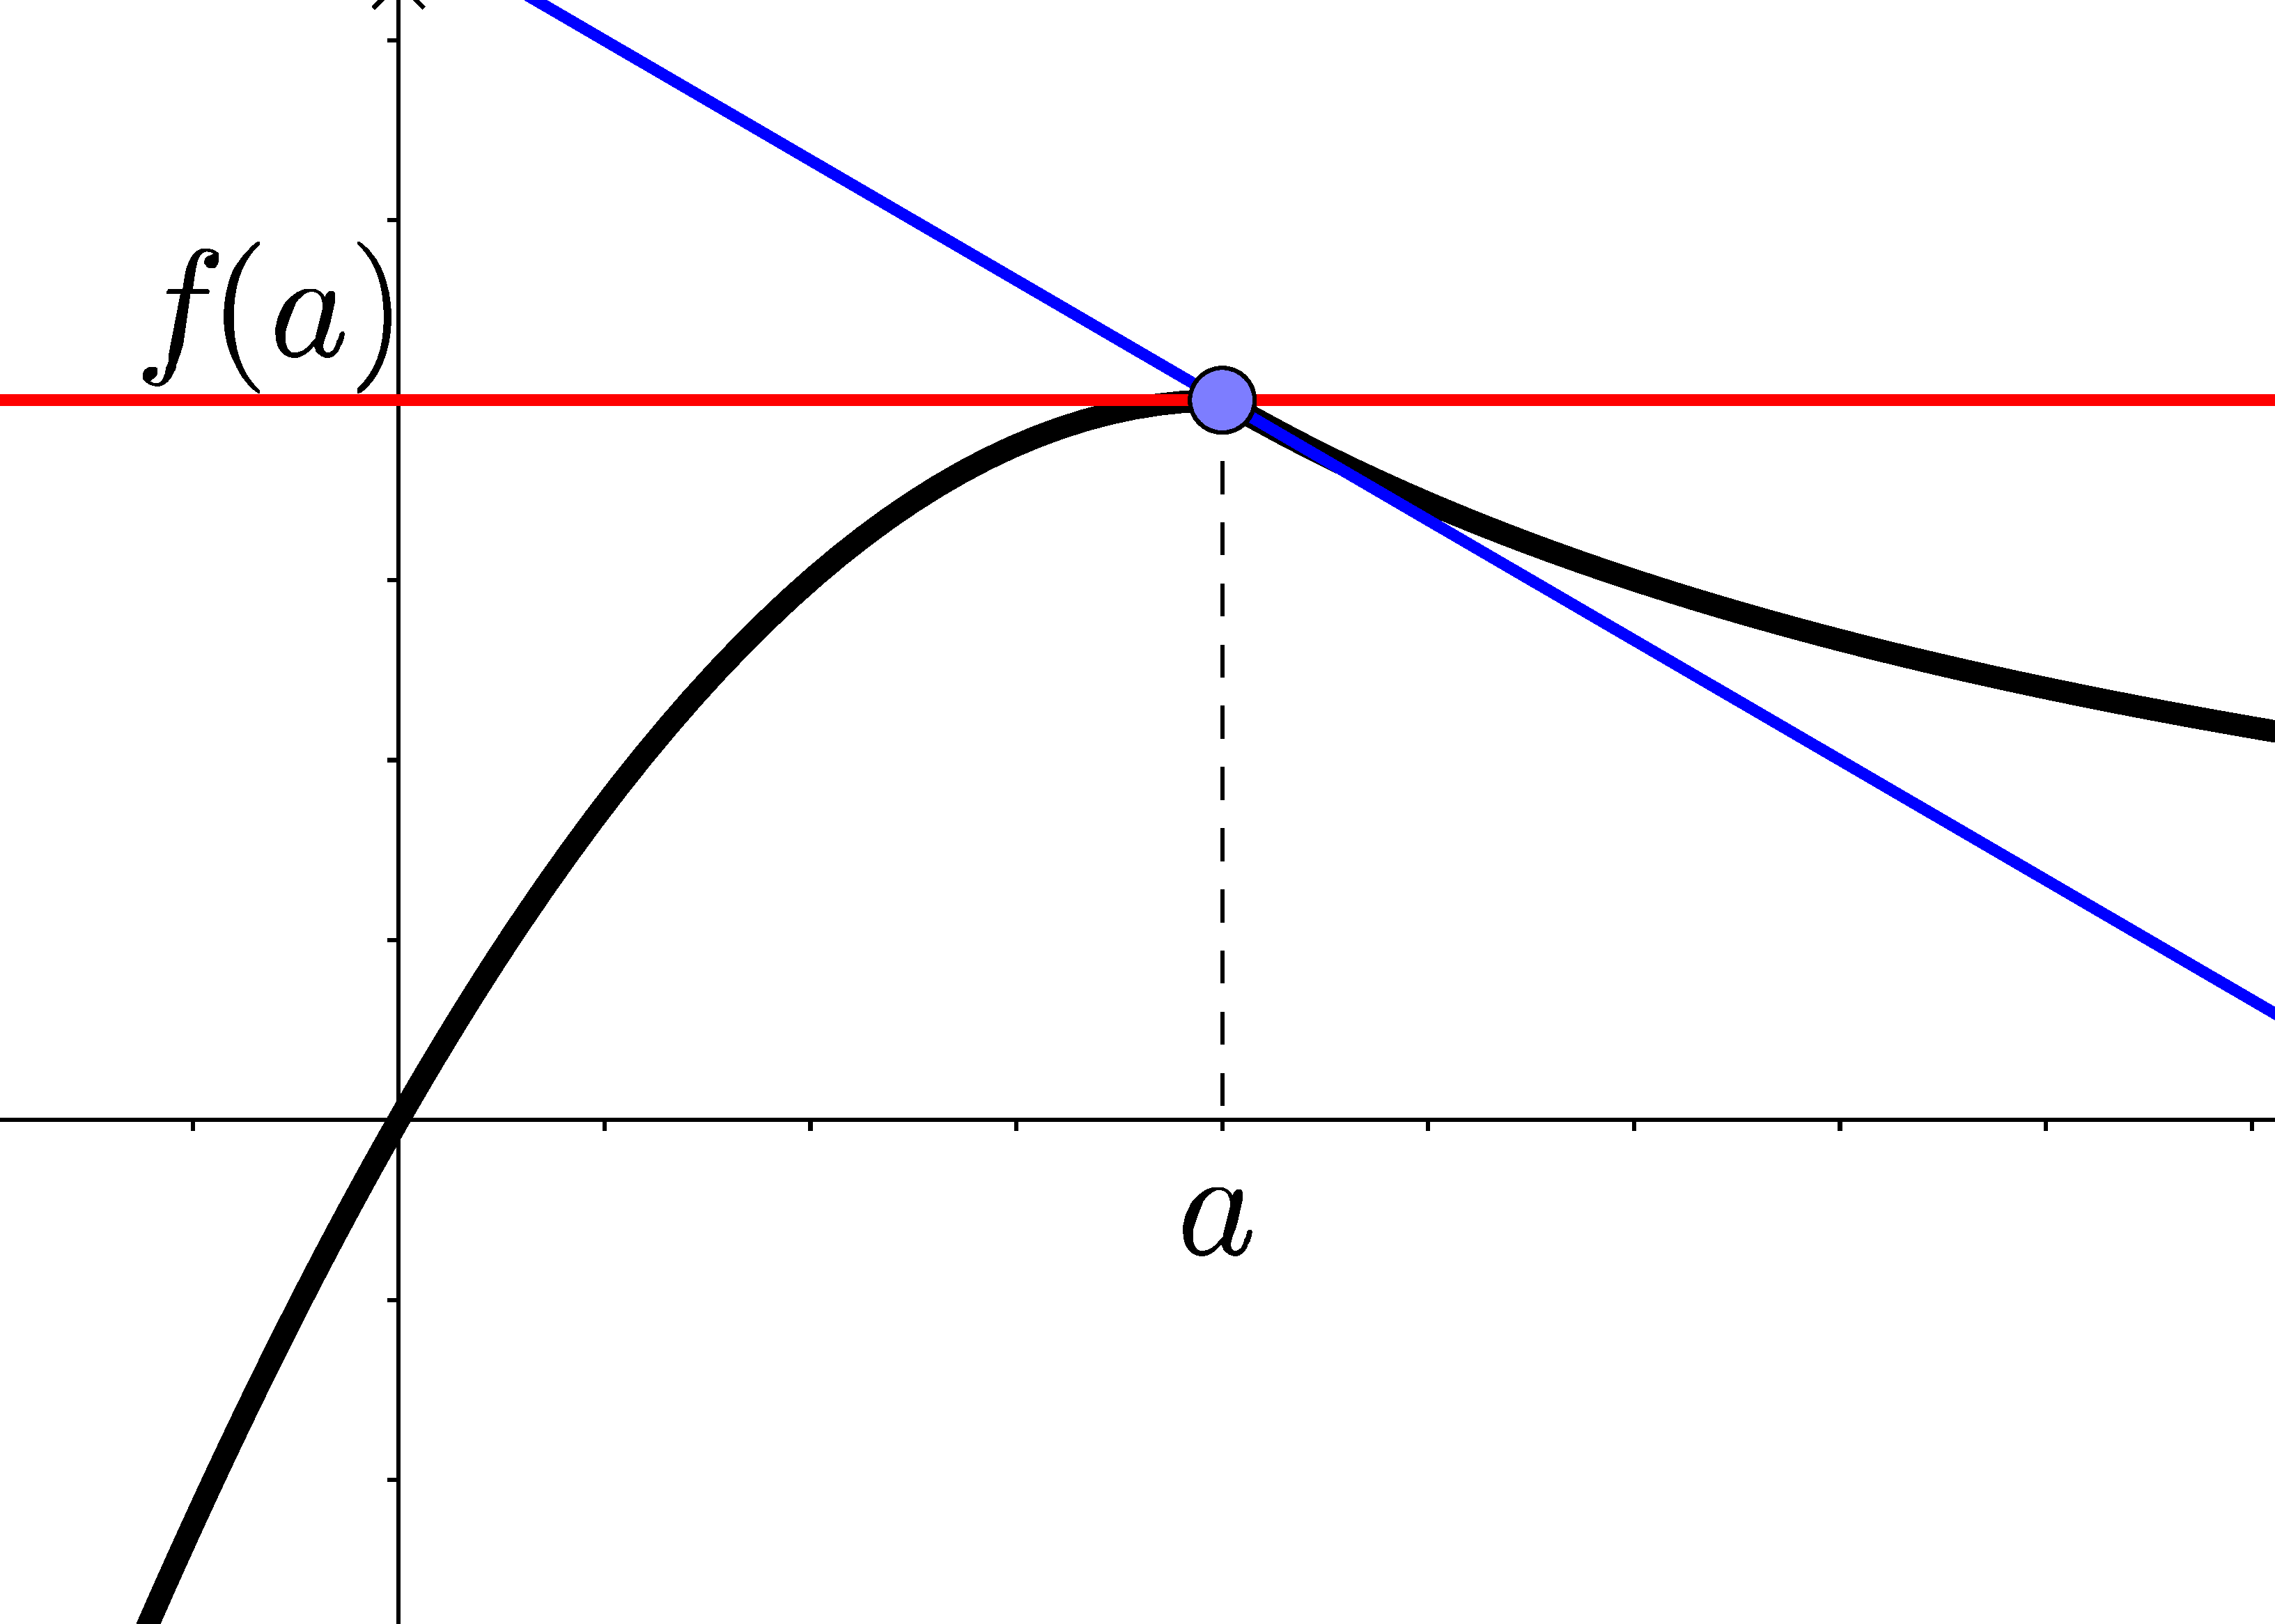
\includegraphics[width=0.9\textwidth]{img-07/puntangulos}
	\end{minipage}
\end{center}
	
	Per a que una funció sigui derivable, ha d'existir el límit anterior. Això passa si la funció és suau o arrodonida, és a dir, no presenta punts angulosos com ara la figura de la dreta.
\end{theorybox}

\begin{resolt}{Utilitza la definició de derivada per calcular la derivada de la funció $f(x) = 3x^2 - 5x + 2$ en el punt d'abscissa $x = 1$.}
	Utilitzam la definició de derivada Eq. (\ref{eq:defderiv}) quan $a=1$:
	\begin{equation*}
	f'(1)  = \limx[h]{0}\frac{f(1+h)-f(1)}{h}
	\end{equation*}
	Necessitam calcular $f(1)=0$, $f(1+h) = 3(1+h)^2 - 5(1+h) + 2$; si substituïm, el límit ens queda:
	\begin{equation*}
	f'(1)  = \limx[h]{0}\frac{3(1+h)^2 - 5(1+h) + 2-0}{h}=\limx[h]{0}\frac{h+3h^2}{h}=1
	\end{equation*}
	on hem simplificat el numerador i resolt la indeterminació $0/0$.
\end{resolt}


\begin{mylist}
	 \exer  En llançar un objecte verticalment cap amunt l'altura (en metres) $y$, que aconsegueix als $x$ segons ve donada per la funció: $y = 40x- 5x^2$
	 
	 \begin{tasks}
	 	\task   Escriu una taula de valors i dibuixa la gràfica de la funció. Té sentit per a valors de $x$ menors que 0? I majors a 8?
	 	%
	 	\task Calcula la velocitat mitjana en els intervals: [0, 2], [0, 8], [1, 4], [4, 8] i [1, 8]. 
	 	%
	 	\task Quina és l'altura màxima aconseguida per l'objecte?
	 	%	 
	 \end{tasks}
 
 \answers{[Solució gràfica. No té sentit per a valors negatius ni per a valors majors de 8. Només ha
 	sentit per $0 \leq x \leq 8$,
 	$v_m [0,2] = 30$ m/s, $v_m[0,8] = 0$ m/s, $v_m [1,4] = 15$ m/s, $v_m [4,8] = - 20$ m/s, $v_m [1,8] = - 5$  m/s,
 	c) $y(4) = 80$ m.]}

\exer Utilitza la definició de derivada per calcular la derivada de la funció $y = x^3$ en el punt $x = 2$.
\answers{$f'(2)=\limx[h]{0} \dfrac{(2+h)^3 - 2^3}{h}=\limx[h]{0} \dfrac{h\,(h^2+6h+12)}{h}=12$}

\exer Utilitza la definició de derivada per calcular la derivada de la funció $y = \sqrt{x} $ en $x = 1$.
\answers{$f'(1)=\limx[h]{0} \dfrac{\sqrt{1+h}-\sqrt{1}}{h}=\limx[h]{0} \dfrac{(\sqrt{1+h}-1)\cdot (\sqrt{1+h}+1)}{h ((\sqrt{1+h}+1))}= \dfrac{h}{h ((\sqrt{1+h}+1))}=\frac{1}{2}$}


\exer Utilitza la definició de derivada per calcular la derivada de la funció $y = \dfrac{1}{x^2}$ en $x = 4$.
\answers{$f'(4)=\limx[h]{0} \dfrac{\frac{1}{(4+h)^2}-\frac{1}{4^2}}{h}=\limx[h]{0} \dfrac{-\frac{h(h+8)}{16(h+4)^2}}{h}=-\dfrac{1}{32}$}


\exer  Dóna un exemple de funció no derivable i que sí sigui contínua.
\answers{Qualsevol funció que presenti punxes, per exemple la funció valor absolut $y=|x|$ no és derivable a $x=0$.}


\end{mylist}

\begin{theorybox}[Funció derivada]
	
	Hem vist que la derivada en un punt $f'(a)$ és un nombre que proporciona el pendent de la recta tangent.
	
	La funció derivada $f'(x)$ dóna el valor de la derivada per un punt $x$ qualsevol. Per exemple:
	
	Si ens diuen que la funció derivada $f'(x)=2x$, aleshores tenim una ``regla'' per trobar tots els pendents. Si volem el pendent per a $x=0$  $f'(0)=2\cdot 0=0$, el pendent per a $x=-3$  $f'(0)=2\cdot (-3)=-6$, etc. 
	
	
	$f'(x)$ és pot obtenir a través de la definició  \ref{eq:defderiv} tot i que, com veurem, serà més còmode a partir de les regles de derivació.
\end{theorybox}


\begin{mylist}


\exer Representa gràficament la funció 
$y=\left\{ \begin{array}{ll} 
	x+2 & 0\leq x < 2  \\ 
	4   & 2 \leq x < 4 \\ 
	-\frac{x}{2}+6 & x\geq 4
\end{array} \right.$. En una altra gràfica representa la seva funció derivada.

\answers{\mbox{}\par 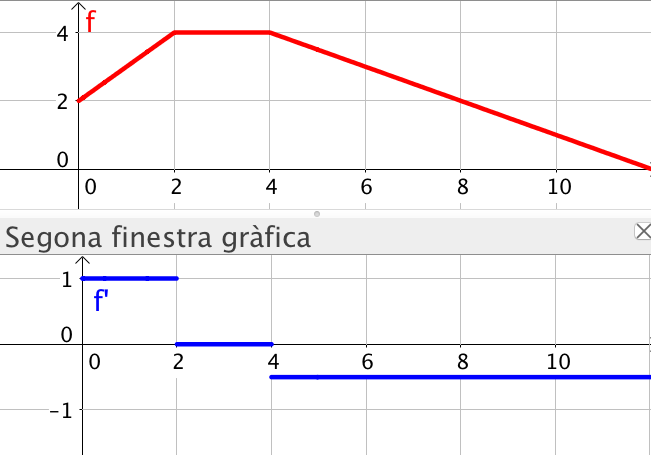
\includegraphics[width=0.4\textwidth]{img-sol/t7-11}}

\exer Sobre la funció $y=f(x)$ de la figura dibuixa la recta tangent en els punts $x=1,\,1.5,\,4,\,5,\,7$. En els eixos de la dreta esbossa la gràfica aproximada de la seva funció derivada.

\begin{center}
\includegraphics*[width=0.4\textwidth]{img-07/chap-deriv-atrossos1}
\includegraphics*[width=0.4\textwidth]{img-07/chap-deriv-atrossos2}
\end{center}

\answers{\mbox{}\par 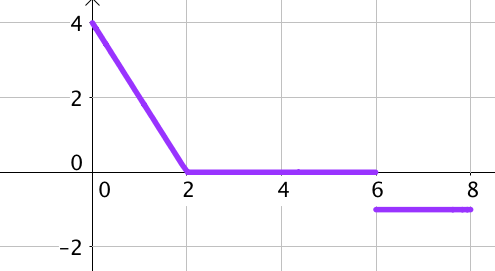
\includegraphics[width=0.4\textwidth]{img-sol/t7-12}}

\end{mylist}

\begin{minipage}{0.8\textwidth}
	\begin{mylist}
		
		\exer  Des d'un avió nodrissa es deixa anar un avió experimental que el seu impulsor s'encén a la màxima potència i roman encès 20 segons. La distància que separa a l'avió experimental de l'avió nodrissa ve donada per 
		$d = 0'3 t^4$. Calcula la velocitat de l'avió experimental als 3, 4, 7 i 10 segons d'haver estat deixat anar.
		
		\answers{ $d’ = 1,2 t^3$; $v(3) = 32,4$ m/s; $v(4) = 76,8$ m/s; $v(7) = 411,6$ m/s; $v(10) = 1200$ m/s.}
		
		\exer  Caiguda lliure d'una pilota. En la figura es mostren, mitjançant fotografia estroboscòpica\footnote{ Un llum estroboscòpica és un instrument que il·lumina una escena durant intervals regulars de temps. 
			Si utilitzem aquest tipus de llum sobre un moviment repetitiu, com la rotació d'una roda, i l'interval coincideix amb un període complet de moviment, l'objecte semblarà estàtic a l'observador.}, 
		les posicions de la pilota a intervals regulars de temps: per a  t = 1, 2, 3, 4, 5, ..., l'espai recorregut és proporcional a 1, 4, 9, 16, 25, ..., etc. 
		Calcula la funció de posició  $y=f(t)$, i calcula la velocitat i l'acceleració derivant la funció de posició.
		
		\answers{$y = f(t) = t^2$; $y' = v = 2t$; $a = y'' = 2$}
		
		
	\end{mylist}
\end{minipage}
\begin{minipage}{0.2\textwidth}
	\begin{center}
		\includegraphics*[width=0.86in, height=2.91in, keepaspectratio=false]{img-07/image58}
	\end{center}
\end{minipage}
 
\begin{mylist}
	\begin{comment}
\exer  En caure un cos en el buit la distancia $d$ (en metres), recorreguda als $t$ segons ve donada aproximadament per l'expressió: $d=5t^2$. 
(L'expressió és  $d = \frac{1}{2} g t^2$, on $g$ és l'acceleració de la gravetat terrestre, aproximadament de 9'8):


\noindent a) A quina velocitat arribarà al terra una persona que en un incendi es llanci a la lona dels bombers i tarda 4 segons a arribar a ella?

\noindent b) A quina velocitat arribarà si es llança des d'una altura de 10 metres?


\exer  Un vehicle espacial desenganxa d'un planeta amb una trajectòria donada per: $y = 50x  - 0'2x^2$ ($x$ i $y$ en km). La direcció del vehicle ens la proporciona la recta tangent en cada punt. 
Determina la direcció del vehicle quan està a 2 km de distància sobre l'horitzó.
\end{comment}


\begin{comment}
\exer  Representa gràficament la funció $y = 2$, i determina la seva derivada per a  $x$ = 1, 2, 3... $a$. Quant val? És sempre la mateixa? Ocorrerà el mateix per a qualsevol recta horitzontal $y=k$?
\end{comment}



\exer  Dibuixa una funció qualsevol i un punt qualsevol sobre la funció $f(a)$. Dibuixa també un segment sobre l'eix d'abscisses amb origen en  $a$ i longitud $h$. 
Interpreta de nou la definició de derivada en un punt basant-te en aquesta figura.


\exer  Calcula la derivada de la funció $y= x^2 - x+ 1$ en el punt $x=1$ mitjançant la definició amb límit. 
Repeteix el càlcul per un punt arbitrari $x=a$. 
Calcula mitjançant l'expressió resultant $f'(1)$, $f'(2)$, $f'(12)$, $f'(5.43)$ i $f'(-7)$.
\answers{$f'(a)=\limx[h]{0} {\dfrac{(a+h)^2-(a+h)+1 -(a^2-a+1)}{h}=\limx[h]{0} \dfrac{h\,(2a+h-1)}{h}=2a-1}$\par 
$f'(1)=1$, $f'(2)=3$, $f'(12)=23$, $f'(5.43)=9.86$ i $f'(-7)=-15$. En general, la funció derivada, $f'(x)=2x-1$.}

\end{mylist}

 
 
%%%%%%%%%%%%%%%%%%%%%%%%%%%%%%%%%%%%%%%%%%%%%%%%%%%%%%%%%%%%%%%%%%%%%%%%%%%%%%%%%%%%%%%%%%%%%%%%%%%%%%%%%%%%%%%%%%%%%%%%%


\section{Regles de derivació}

\begin{theorybox}

	\begin{minipage}{0.33\textwidth}
		\centering\videonw{184}{Taula de derivades}
	\end{minipage}
\begin{minipage}{0.33\textwidth}
	\centering\videonw{185}{Regla de la cadena}
\end{minipage}
\begin{minipage}{0.33\textwidth}
	\centering
	\videonw{186}{Producte i quocient de funcions}
\end{minipage}
	

\end{theorybox}


\pagebreak
 
\begin{center}
\textbf{Taula de derivades}
	\setlength\LTleft{0pt}
	\setlength\LTright{0pt}
	\fontsize{10.5}{11}
	\def\arraystretch{1.01}
	\begin{longtable}[h]{|p{0.2\textwidth}|p{0.25\textwidth}||p{0.2\textwidth}|p{0.25\textwidth}|}
		\hline
		\multicolumn{2}{|c||}{\cellcolor{lightgray}\noindent\textit{Funcions elementals}} &  \multicolumn{2}{|c|}{\cellcolor{lightgray}\noindent\textit{Funcions compostes}} \\  [1.5ex] \hline
		\cellcolor{lightgray}\noindent$y=f(x)$ & \cellcolor{lightgray}\noindent$y'=f'(x)$ & \cellcolor{lightgray}\noindent$y=f(g(x))$ & \cellcolor{lightgray}\noindent$y'=f'(g(x))\cdot g'(x)$  \\  [1.5ex] \hline
		$y=k$ & $y'=0$ &  &  \\  [1.5ex] \hline
		$y=x$ & $y'=1$ &  &  \\ [1.5ex] \hline
		$y=x^n$ & $y'=n x^{n-1}$ &   $y=[g(x)]^n$ & $y'=n [g(x)]^{n-1} \cdot g'(x)$   \\ [1.5ex] \hline
		$y=\sqrt{x}$ & $y'=\dfrac{1}{2 \sqrt{x}}$ &   $y=\sqrt{g(x)}$ & $y'=\dfrac{1}{2 \sqrt{g(x)}}\cdot g'(x)$  \\ [1.5ex] \hline
		$y=\sin x$ & $y'=\cos x$ &   $y=\sin g(x)$ & $y'=\cos g(x) \cdot g'(x)$   \\ [1.5ex] \hline
		$y=\cos x$ & $y'=-\sin x$ &   $y=\cos g(x)$ & $y'=-\sin g(x) \cdot g'(x)$   \\ [1.5ex] \hline
		$y=\mathrm{tg}\, x$ & $y'=\dfrac{1}{\cos^2 x}=$ \newline $\,\,=1+\mathrm{tg}^2\, x$ &   $y=\mathrm{tg}\, g(x)$ & $y'=\dfrac{1}{\cos^2 g(x)} \cdot g'(x)=$ \newline $\,\,=[1+\mathrm{tg}^2\, g(x)] \cdot g'(x)$   \\ [1.5ex] \hline
		$y=\mathrm{cotg}\, x$ & $y'=\dfrac{-1}{\sin^2 x}$ &   $y=\mathrm{cotg}\, g(x)$ & $y'=-\dfrac{1}{\sin^2 g(x)} \cdot g'(x)$   \\ [1.5ex] \hline
		$y=\arcsin x$ & $y'=\dfrac{1}{\sqrt{1-x^2}}$ &   $y=\arcsin g(x)$ & $y'=\dfrac{1}{\sqrt{1-g^2(x)}} \cdot g'(x)$ \\ [1.5ex] \hline
		$y=\arccos x$ & $y'=\dfrac{-1}{\sqrt{1-x^2}}$ &   $y=\arccos g(x)$ & $y'=\dfrac{-1}{\sqrt{1-g^2(x)}} \cdot g'(x)$ \\  [1.5ex] \hline
		$y=\mathrm{arctg}\, x$ & $y'=\dfrac{1}{1+x^2}$ &   $y=\mathrm{arctg}\, g(x)$ & $y'=\dfrac{1}{1+g^2(x)} \cdot g'(x)$ \\  [1.5ex] \hline
		$y=e^x$ & $y'=e^x$ &   $y=e^{g(x)}$ & $y'=e^{g(x)} \cdot g'(x)$   \\  [1.5ex] \hline
		$y=a^x$ & $y'=a^x \, \ln a$ &   $y=a^{g(x)}$ & $y'=a^{g(x)} \, \ln a \cdot g'(x)$   \\  [1.5ex] \hline
		$y=\ln x$ & $y'=\dfrac{1}{x}$ &   $y=\ln{g(x)}$ & $y'=\dfrac{1}{g(x)} \cdot g'(x)$  \\ [1.5ex] \hline
		$y=\log_a x$ & $y'=\dfrac{1}{x}\cdot\dfrac{1}{\ln a}$ &   $y=\ln{g(x)}$ & $y'=\dfrac{1}{g(x)}\cdot\dfrac{1}{\ln a} \cdot g'(x)$  \\ [1.5ex] \hline
	\end{longtable}
\vspace{-0.5cm}

\textbf{Regles de derivació:}
\end{center}

\begin{itemize}

	\item Derivada de constant per funció:
	$y=k \, f(x)$   $\rightarrow$   $y'=k \, f'(x)$
	
	%$y=5 \sin x$  $\rightarrow$   $y'=5 \cos x$
	
	
	\item Derivada de sumes / restes:
	$y=f(x)+g(x)$   $\rightarrow$   $y'=f'(x)+g'(x)$
	
	%$y=5 e^x - 2 \ln x$   $\rightarrow$   $y'=5 e^x - \dfrac{2}{x}$
	
	
	\item Regla de la cadena:
	$y=f(g(x))$   $\rightarrow$   $y'=f'(g(x))\cdot g'(x)$
	\begin{center}
	$y=\ln (\mathrm{tg}\, x)$   $\rightarrow$   $y'=\dfrac{1}{\mathrm{tg}\, x} \cdot \dfrac{1}{\cos^2 x}$
	\end{center}
	
	\item Derivada d'un producte:
	$y=f(x)\cdot g(x)$   $\rightarrow$   $y'=f'(x)\cdot g(x)+f(x)\cdot g'(x)$
	\begin{center}
	$y=x^2 \sin x$   $\rightarrow$   $y'=2x\sin x + x^2 \cos x = x (2 \sin x + x \cos x)$
	\end{center}
	\item Derivada d'un quocient:
	$y=\dfrac{f(x)}{g(x)}$   $\rightarrow$   $y'=\dfrac{f'(x)\cdot g(x)-f(x)\cdot g'(x)}{g^2(x)}$
	\begin{center}
	$y=\dfrac{x^2}{x^3-4}$   $\rightarrow$   $y'=\dfrac{2x \cdot (x^3-4)-x^2 \cdot (3x^2)}{(x^3-4)^2}=\dfrac{-x^4-8x}{(x^3-4)^2}$
	\end{center}
	
\end{itemize}


%%%%%%%%%%%%%%%%%%%%%%%%%%%%%%%%%%%%%%%%%%%%%%%%%%%%%%%%%%%%%%%%%%%%%%%%%%%%%%%%%%%%%%%%%%%%%%%%%%%%%%%%%%%%%%%%%%%%%%%%%


 
\begin{mylist}

\exer \spen Completa en el teu quadern la següent taula amb les derivades:


\begin{tabular}{|p{0.6in}|p{0.5in}|p{0.5in}|p{0.5in}|p{0.5in}|p{0.5in}|p{0.5in}|p{0.6in}|} \hline 
	\textbf{Funció $f(x)$} & $x^3$ & $ 2$ & $ x^2$ & $ x$ & $ k$ & $ 2x+ 3$ & $ 2 x^2+ 3x$ \\ \hline 
	\textbf{Derivada $f'(x)$} & $3x^2$ &  &   &   &   &  & \\ \hline 
\end{tabular}

\answers{$3x^2$, $0$, $2x$, $1$, $0$, $2$, $4x+3$}

\exer \mental  Escriu les funcions derivades de les funcions següents: 

\begin{tasks}(3)
	\task $f(x) = x^{24}$ \task  $g(x) = 6x^{10}$ \task  $h(x) = {2 \over 13} x^{13}$ \task  $j(x) = 3x^4 - 5x^2 + 7$ \task  $p(x) = 5x^3- x$
\end{tasks}

\answers{[$f'(x)=24 x^{23}$, $g'(x)=60 x^9$, $h'(x)=2 x^{12}$, $j'(x)=12 x^3 -10x$, $p'(x)=15x^2-1$]}

\exer Calcula les derivades de les següents funcions:


\begin{tasks}(3) 
	\task $f(x) = 4 \sqrt[3]{x^2}$ 
	\task $f(x)=\dfrac{x\sqrt[4]{x}}{\sqrt{3x}}$
	\task $f(x)=5\sqrt{x}+\dfrac{2}{x}- \dfrac{3}{x^2}$
\end{tasks}
\answers{[$f'(x)=\dfrac{8}{3}\dfrac{1}{\sqrt[3]{x}}$, $f'(x)=\frac{\sqrt{3}}{4\sqrt[4]{x}}$, $f'(x)=\dfrac{5}{2\sqrt{x}}-\dfrac{2}{x^2}+\dfrac{6}{x^3}$]}

\exer  Ja hem obtingut la derivada de $y=\sqrt{x} =x^{\frac{1}{2} } $. Utilitza-la per obtenir la derivada en \linebreak $x$ = 1, 4, 5... Pots obtenir la derivada en $x$ = 0? Raona la resposta.
\answers{$y'=\dfrac{1}{2\sqrt{x}}$. $y'(1)=\dfrac{1}{2}$; $y'(4)=\dfrac{1}{4}$; $y'(5)=\dfrac{1}{2\sqrt{5}}$; etc. No existeix la derivada a $x=0$ perquè valdria $+\infty$}

\begin{comment}
\exer Un determinat gas ocupa un volum de 2 m$^3$ a una pressió de 5 Newtons per m$^2$. Segons la llei de Boyle a cada pressió exercida sobre el gas correspon un volum donat per $V = 10/P$. Quina és la taxa de variació instantània del volum quan la pressió és de 10 N/m$^2$. I quan és de 20 N/m$^2$? És la meitat?  
\end{comment}

\exer[1] Calcula les derivades simplificades utilitzant la regla de la cadena per funcions compostes

\begin{tasks}(2)
	\task $f(x)=(x^2+x+1)^3$ 
	\task $f(x)=\left(\ln(2x+3)\right)^5$
	\task $f(x)=(3 x^4+7)^5$
	\task $f(x)=\sqrt{3x^2+2x+7}$
	\task $f(x)=e^{-x^2}$
	\task $f(x)=\sin \left( \ln x \right)$
	\task $f(x)=\ln (\sin \sqrt{x})$
	\task $f(x)=\ln \left( \mathrm{tg}\, (x^2+1) \right)$
\end{tasks}
\answers[cols=1]{[$y'=3(x^2+x+1)^2\,(2x+1)$, $y'=10\ln^4 (2x+3) \dfrac{1}{2x+3}$, $y'=60(3x^4+7)^4 \,x^3$, $y'=\dfrac{3x+1}{\sqrt{3x^2+2x+7}}$, $y'=-2x \,e^{-x^2}$, $y'=\cos (\ln x)\,\dfrac{1}{x}$, $y'=\dfrac{1}{2\sqrt{x}\,\tg \sqrt{x}}$, $y'=\dfrac{2x \left[1+\tg^2(x^2+1)\right]}{\tg(x^2+1)}$]}

\end{mylist}

\begin{example}
	  a)  $f(x)=(x^2+x+1)^3$ \qquad $\rightarrow$
		 
		\quad $f'(x)=3(x^2+x+1)^2 \cdot (2x+1+0) = 3(2x+1)\,(x^2+x+1)^2$
	 
		 b) $f(x)=\left(\ln(2x+3)\right)^5$	\qquad $\rightarrow$
		 
		\quad $f'(x)=5\left(\ln(2x+3)\right)^4 \cdot \frac{1}{2x+3} \cdot 2 = 10\ln^4 (2x+3) \dfrac{1}{2x+3}$	
	 
\end{example}


\begin{mylist}
	
 
\exer  Calcula les derivades simplificades de les següents funcions:

\begin{tasks}(2)
	\task $y = (x^5 - 7x^3)^{12}$  \task $y = (3x^3 - 5x^2)^7$  \task $y=\sqrt{\left(4x^{5} -8x^{3} \right)^{5} } $    \task $y=\sqrt[{3}]{\left(2x^{2} +4x^{7} \right)^{4} } $
\end{tasks} 

\answers{[$y' = 12(x^5 - 7x^3)^{11} (5x^4-21x^2)$, $y' = 7(3x^3 - 5x^2)^6 (9x^2-10x)$, $y=\dfrac{1}{2\sqrt{\left(4x^{5} -8x^{3} \right)^{5} }} \cdot 5 \left(4x^{5} -8x^{3} \right)^{4} \cdot (20 x^4 - 24x^2) $, $y'=\dfrac{4}{3}\sqrt[{3}]{\left( 2x^{2} +4x^{7} \right) } \cdot (4x+28x^6) $]}
	
\exer  Calcula les derivades simplificades de les següents funcions:

\begin{tasks}(3)
	\task $y = \sin(x^5 - 7x^3)$ 
	\task  $y = \sin^7(3x^3 - 5x^2)$   
	\task  $y=\sqrt[{3}]{\sin\left(2x^{2} +4x^{7} \right)^{4} } $
\end{tasks}

\answers{[$y' = (5x^4-21 x^2) \cos(x^5 - 7x^3)$,   $y' = 7 \sin^6(3x^3 - 5x^2) \cdot \cos(3x^3 - 5x^2) \cdot (9x^2-10x)$,
	  $y'=-\dfrac{4(2x^{2} +4x^{7})^3 (4x+28x^6) \cos  \left(2x^{2} +4x^{7} \right)^{4} }{\sqrt[{3}]{\sin^2  \left(2x^{2} +4x^{7} \right)^{4} } }$ ]}

\exer  Calcula les derivades simplificades de les següents funcions:

\begin{tasks}(3)
	\task  $y = \cos(e^{x^5} + 4x^3)$   \task  $y = (\cotg(5x^3 - 3x^2))^4$
	\task  $y = \tg(7x^5 - 3x^3)^2$   
\end{tasks}

\answers{[ $y' = -(5x^4 e^{x^5}+12x^2) \sin(e^{x^5} + 4x^3)$,  $y' = -4(\cotg(5x^3 - 3x^2))^3 \cdot \dfrac{15x^2-6x}{\sin^2(5x^3 - 3x^2)}$,
  $y' = \left[ 1+\tg^2(7x^5 - 3x^3)^2 \right] \cdot 2 (7x^5-3x^3)\cdot (35x^4-9x^2)$ ]}

\exer[1] Calcula les derivades simplificades  utilitzant la regla del producte

\begin{tasks}(2)
	\task $f(x)=x\cdot \sin x + x^2\cdot \cos x$
	\task $f(x)=x\cdot \ln x$
	\task $f(x)=3^x\cdot \mathrm{tg}\, x $
	\task $f(x)=(x^2+1)\cdot e^x$
	\task $f(x)=5x^2\cdot \mathrm{arctg}\, x$
	\task $f(x)= \ln (x+1) \cdot \sin x^2$
\end{tasks}
\answers[cols=1]{[$y'=(1-x^2)\sin x+3x\cos x$, $y'=\ln x +1$, $y'=3^x \left( \tg^2 x + \ln 3 \tg x + 1 \right)$, $y'=(x+1)^2 e^x$, $y'=10x\,\arctg x + \dfrac{5x^2}{1+x^2}$, $y'=\dfrac{\sin x^2}{x+1} + 2x\ln x\cos x^2$]}


\end{mylist}

\begin{example}
	a) $f(x)=x\cdot \sin x + x^2\cdot \cos x$ \qquad $\rightarrow$
	
	\quad $f'(x)=1\cdot \sin x + x\cdot \cos x + 2x\cdot \cos x+ x^2\cdot (-\sin x)=(1-x^2)\sin x+3x\cos x$
\end{example}

\begin{mylist}
		
	\exer[1] Calcula les derivades simplificades utilitzant la regla del quocient
	
	\begin{tasks}(2)
		\task $f(x)=\dfrac{\ln x}{x}$
		\task $f(x)=\dfrac{\cos x}{\sin x}$
		\task $f(x)=\dfrac{x+1}{x-1}$
		\task $f(x)=\dfrac{\sqrt{x}-1}{x^2}$
		\task $f(x)=\dfrac{1-\sin x}{1+\sin x}$
		\task $f(x)=\dfrac{x^2-x-1}{x^2-1}$
		\task $f(x)=\dfrac{(x-1)\cdot(x-2)}{(x-3)\cdot (x-4)}$
		\task $f(x)=\dfrac{1}{x^3+3x^2+3x-1}$
	\end{tasks}
\answers[cols=1]{[$y'=\dfrac{1 - \ln x  }{x^2}$, $y'=\dfrac{-1}{\sin^2 x}$, $y'=\dfrac{-2}{(x-1)^2}$, $y'=\dfrac{4x-3\sqrt{x^3}}{2x^4}$, $y'=\dfrac{-2\cos x}{(1+\sin x)^2}$,  $y'=\dfrac{x^2+1}{(x^2-1)^2}$, $y'=\dfrac{-4 \; x^{2} + 20 \; x - 22}{(x-3)^2 (x-4)^2}$, $y'=\dfrac{-3 \; x^{2} - 6 \; x - 3}{(x^3+3x^2+3x-1)^2}$]}

\end{mylist}
\begin{example}
	a) $f(x)=\dfrac{\ln x}{x}  \quad \rightarrow \quad f'(x)=\dfrac{\frac{1}{x}\cdot x - \ln x \cdot 1 }{x^2}=\dfrac{1 - \ln x  }{x^2}$ 
	\vspace{0.5cm}
\end{example}


\begin{mylist}
	
	\exer Calcula les derivades utilitzant les regles de derivació
	
	\begin{tasks}(2)
		\task $f(x)=x\cdot e^{1 \over x^2}$
		\task $f(x)=\dfrac{e^{4x}+e^{-x}}{2x}$
		\task $f(x)=\dfrac{\ln (x^2+1)}{2x-1}$
		\task $f(x)= \left(\cos (2x) \right)^2 \cdot e^{-(2x+1)^2}$
	\end{tasks}

\answers{[$f'=(1-\dfrac{2}{x^2}) e^{1\over x^2}$, $f'=\dfrac{(4x-1)e^{4x}-(x+1)e^{-x}}{2x^2}$, $f'=\dfrac{2x}{(x^2+1)(2x-1)}.\dfrac{2\ln(x^2+1)}{(2x-1)^2}$, 
	$f'=-4 e^{-(2x+1)^2} \cos(2x) \cdot \left[ \sin(2x)+(2x+1) \cos(2x) \right]$ ]}

	
	 
	\exer  Calcula les derivades de les següents funcions:
	
	\begin{tasks}(2)
	\task $y = (x^2 + 3) \cdot (6x^6 - 5)$ 
	\task $y = (7x^3 - 1) \cdot (5x^4 + 4)$ 
	\task $y=\sqrt{x} \cdot (x^{3} -5x)$
	\end{tasks}

\answers{[$y'=48x^7+108 x^5-10x$, $y'=256x^6-20x^3+84x^2$, $y'=\frac{\sqrt{x}}{2} \left(7x^2-15 \right)$]}
 
	\exer  Calcula les derivades de les següents funcions:
	\begin{tasks}(2)
	\task $y=\dfrac{x-1}{x+3} $  
	\task $y=\dfrac{2x^{3} -5x^{2} }{6x^{4} -2x^{3} } $ 
	\task $y=\dfrac{\sqrt{x^{3} } }{x+2} $
	\task $y=\dfrac{\sqrt[{3}]{x^{2} } \cdot \sqrt{x} }{x^{3} +5} $
    \task $y=\dfrac{(x^{4} -2)\cdot \sqrt{x} }{\sqrt[{4}]{x^{5} } } $ 
	\task $y=\dfrac{\sqrt[{6}]{x^{11} } }{x+2} $ 
	\end{tasks}
	
	\answers{[$y'=\dfrac{4}{(x+3)^2}$, $y'=\dfrac{-6x^2+30x-5}{2(3x^2-x)^2}$, 
		$y'=\dfrac{\sqrt{x} (x+6)}{2(x+2)^2}$, $y'=\dfrac{\sqrt[6]{x} (35-11x^3)}{6(x^3+5)^2}$, $y'=4x^3\cdot x^{-3/4}+ (x^4-2)\cdot(-3/4)\cdot x^{-7/4} =\dfrac{13x^4+6}{4\sqrt[4]{x^7}}$, $y'=\dfrac{\sqrt[6]{x^5} (5x+22)}{6(x+2)^2}$]}
	
	\begin{comment}
	\exer  Calcula les derivades de les següents funcions:
	
	\begin{tasks}(2)
	\task $y=\sqrt{\frac{3x^{2} -5x}{2x^{3} +7} \left(x^{4} -6x^{3} \right)^{2} } $ 
	\task $y=\sqrt{\frac{(x^{2} +3)(x^{2} -7)}{x^{3} -5} } $  
	\task $y=\sqrt{\left(\frac{5x^{2} +3x}{8x^{3} -2x^{2} } \right)^{3} } $  
	\task $y=\sqrt[{3}]{3+\sqrt{x-\frac{2}{x^{3} } } } $
		\end{tasks}
	\end{comment}
	
		
	\end{mylist}

	\begin{theorybox}
		
	\textbf{$\bullet$ Derivades amb logaritmes:}
	
	En comptes de derivar directament la funció $y=\ln \dfrac{\sqrt{x^2+1}}{3x+5}$, resulta més senzill aplicar les propietats dels logaritmes de la pàgina \pageref{eq:proplog}. Separam la funció en diferents logaritmes:
		\[ y=\ln\sqrt{x^2+1} -\ln (3x+5)=\frac{1}{2}\ln (x^2+1) -\ln (3x+5) \]
		ara derivam la darrera expressió fàcilment:
		\[y'=\frac{1}{2} \frac{2x}{x^2+1}  -\frac{3}{3x+5}\]
	
	\textbf{$\bullet$ Derivació logarítmica:}
	
	Ens adonam que la funció $y=x^x$ no és ni potència ni exponencial i, per tant, no tenim cap fórmula per derivar-la. El que feim és prendre logaritmes als dos membres, aplicam les propietats i derivam aplicant la regla de la cadena
			\[ \ln y= \mathbf{x} \cdot \ln x \qquad \rightarrow  \qquad \frac{1}{y} y' = \ln x + x\frac{1}{x} \]
		finalment, aïllam la derivada $y'=x^x \cdot \left(\ln x + 1 \right)$ .
		
	\end{theorybox}

	\begin{mylist}
	
	\exer  Calcula les derivades (Utilitza les propietats dels logaritmes pàg. \pageref{eq:proplog}):
	
	\begin{tasks}(2)
	\task $y = \log (x^5 - 7x^3)^{12}$  \task $y = \log_{2} (3x^3 - 5x^2)^7$  \task $y=\ln \sqrt{\frac{\left(4x^{5} -8x^{3} \right)^{5} }{3x-2} } $   \task  $y=\ln \sqrt[{3}]{\left(2x^{2} +4x^{7} \right)^{4} } $
	\end{tasks}

\answers{[$y'=\dfrac{12}{\ln 10 (x^5-7x^3)}(5x^4-21x^2)$, $y'=\dfrac{7}{\ln 2}\dfrac{9x^2-10x}{3x^3-5x^2}$, $y'=\dfrac{1}{2}\left[ \dfrac{5(20x^4-24x^2)}{4x^5-8x^3} - \dfrac{3}{3x-2} \right]$, $y'=\dfrac{8}{3(x^2+2x^7)}(x+7x^6)$]}
	
	\exer  Utilitza derivació logarítmica per calcular les derivades de les següents funcions:
	\begin{tasks}(3)
		\task $y=x^{x^5-7x^3}$
		\task $y=(x+1)^{3x^3-5x^2}$
		\task $y=x^{(4x^5-8x^3)^5}$
	\end{tasks}
	\answers{[$y'=x^{x^5-7x^3}\cdot \left( (5x^4-21x^2)\ln x + x^4-7x^2 \right)$,  
		     $y'=(x+1)^{3x^3-5x^2}\cdot \left( (9x^2-10x) \ln(x+1) +\frac{3x^3-5x^2}{x+1} \right)$,  
		     $y'=x^{(4x^5-8x^3)^5}\cdot (4x^5-8x^3)^4 \cdot x^2 \cdot \left( 20(5x^2-6)\ln x - 4x^2+8 \right)$]}
	
	\exer Utilitza derivació logarítmica per calcular les derivades de les següents funcions:
		\begin{tasks}(3)
	\task $y=\dfrac{\left(x-1\right)\cdot \left(2x-3\right)}{x+2} $         
	\task $y=\dfrac{\left(3x^{2} +4\right)\cdot \left(4x-2\right)}{7x-1} $  
	\task $y=\dfrac{\left(x+9\right)\cdot \left(2x-3\right)}{\left(x+3\right)\cdot \left(x+2\right)} $
		\end{tasks}
	
	\answers{[$y'=\dfrac{\left(x-1\right)\cdot \left(2x-3\right)}{x+2} \left[ \dfrac{1}{x-1}+\dfrac{2}{2x-3} -\dfrac{1}{x+2}\right]$, 
		   	  $y'=\dfrac{\left(3x^{2} +4\right)\cdot \left(4x-2\right)}{7x-1}\left[ \dfrac{6x}{3x^2+4}+ \dfrac{4}{4x-2} -\dfrac{7}{7x-1} \right]$, 
		      $y'=\dfrac{\left(x+9\right)\cdot \left(2x-3\right)}{\left(x+3\right)\cdot \left(x+2\right)}  \left[ \dfrac{1}{x+9}+\dfrac{2}{2x-3}-\dfrac{1}{x+3}-\dfrac{1}{x+2} \right]$]}
	  
	
	\begin{comment}
	\exer  Utilitzant que la derivada d'y  = i\textit{${c}^{x}$} és \textit{i'}= i\textit{${c}^{x}$}, calcula les derivades de les següents funcions:
	
	
	a)  
	
	
	\exer  Recorda la definició de cosecant: \textit{cosec}(x) = $\frac{1}{sen(x)} $. Demostra que: (\textit{cosec}(x))' = $-\frac{\cos (x)}{sen^{2} (x)} $\textit{ }
	
	\exer  Recorda la definició de la secant: $\sec (x)=\frac{1}{\cos (x)} $. Demostra que: $(\sec (x))'=\frac{sen(x)}{\cos ^{2} (x)} $
	
	\exer  Recorda la definició de cotangent: \textit{cotg}(x) = $\frac{1}{tg(x)} $. Demostra que: (\textit{cotg}(x))' = $-\frac{1}{sen^{2} (x)} $
 

	
	\exer  Calcula les derivades de les següents funcions:
	
	
	\noindent a) $f(x)=tg\frac{1+e^{3x} }{1-e^{3x} } $  b) $f(x)=(2-3x)sh(2-3x)$  c) $f(x)=tg\frac{\sqrt{4-9senx} }{3+2\cos x} $  d) $f(x)=\frac{senx-x\cos x}{\cos x+xsenx} $
	
	
	\exer  Calcula les derivades de les següents funcions:
	
	
	a) y = $arcsen\sqrt{x+1} $   b) $y=\ln (\arccos x)$  c) $y=arctg(e^{2x+3} )$   d) $y=\arccos (sen(\cos x))$
	
	
	\exer  Calcula les derivades de les següents funcions:
	
	
	\noindent a) y = $arcsen\sqrt{\frac{1+senx}{1-senx} } $   b) $y=e^{\arccos \sqrt{x+3} } $  c) $y=sen(arctg\frac{x}{\sqrt{1-x^{2} } } )$  d) $y=\arccos \frac{x}{\sqrt{9-x^{2} } } $
	
	
	\exer  Calcula les derivades de les següents funcions:
	
	
	\noindent a) y = $\arg sh\sqrt{2x+3} $   b) $y=\ln \left(\arg th\left(5x\right)\right)$  c) $y=\arg ch(e^{4x-1} )$   d) $y=\arg sh\left(\arg th\left(x\right)\right)$
	
	 
	
	%%%%%%%%%%%%%%%%%%%%%%%%%%%%%%%%%%%
	
    
	\exer Calcula les derivades de les següents funcions:
	
	a) y = $\ln left( (7x^5 - 2x^3)^12 \cdot (2x + 3) right)$ b) $y=\ln \sqrt{\left(3x^{3} +2x^{2} \right)^{3} } $   c) $y=\ln \sqrt{\frac{4x^{5} -7x}{6x-1} } $   d) $y=\ln \sqrt[{3}]{\left(x^{4} -2x^{5} \right)^{2} } $
	
	
	\exer Calcula les derivades de les següents funcions:
	
	a) $f(x)=\frac{\cos (x)}{3+sen(x^{2} )} $   b) $f(x)=sen(sh^{3} 2x)$  c) $f(x)=ch(sh(5x))$  d) $f(x)=th(2x+3x^{2} )$
	
	
	\exer Calcula les derivades de les següents funcions:
	
	a) $f(x)=9\sqrt{sen^{3} (5x+2)} $  b) $f(x)=\ln \sqrt{\frac{3+2\cos (x)}{3-2\cos (x)} } $  c) $f(x)=ch(sen(5x-2)^{2} )$ d) $f(x)=\ln (\cos ^{2} (x-1))$
	
	
	\exer Calcula les derivades de les següents funcions:
	
	\noindent a) $y = \cos(x^5 - 7x^3)\cdot \sin(x^5 - 7x^3)$ b) $y = \cos^7(3x^3 - 5x^2)\cdot \sin^{5}(3x^3 - 5x^2)$  c) $y = \cos(4x^5 - 8x^3)^5$   d) $y=\sqrt[{3}]{\cos \left(2x^{2} +4x^{7} \right)^{4} }$
	
	 
	\exer Calcula les derivades de les següents funcions:
	
	\noindent a) $f(x)=sen\frac{3+2e^{3x} }{3-2e^{3x} } $  b) $f(x)=(3x-5x^{2} )ch(3x-5x^{2} )$  c) $f(x)=tg\frac{\sqrt{25-14senx} }{4+5\cos x} $  d) $f(x)=\frac{shx-xchx}{chx+xshx} $
	
	
	\exer Calcula les derivades de les següents funcions:
	
	a) $f(x)=\ln \sqrt{e^{2shx-1} } $  b) $f(x)=arcsen\frac{5-3x^{2} }{5+3x^{2} } $ c)$f(x)=7\arccos \frac{4senx+3}{5-2senx} $  d) $f(x)=arcsen\frac{2\cos x}{4senx+3\cos x} $
	
	
	\exer Calcula les derivades de les següents funcions:
	
	a) y = $arcsen(e^{2x-3} )$  b) $y=\sqrt{\ln (\arccos x)} $  c) $y=arctg(\ln \sqrt[{3}]{3x-2} )$  d) $y=arcsen(tg(sen(5x-1)))$
	
	
	\exer Calcula les derivades de les següents funcions:
	
	a) y = $arctg\sqrt{\frac{3+2senx}{3-2senx} } $  b) $y=e^{arcsen\sqrt{2x-5} } $  c) $y=\cos (arcsen\frac{4x-5}{\sqrt{5-3x^{2} } } )$  d) $y=arcsen\frac{2x}{\sqrt{8-x^{2} } } )$
	
	
	\exer Calcula les derivades de les següents funcions:
	
	\noindent a) y = $arctg\sqrt{5x-7} $  b) $y=\ln (\sqrt{arcsen(2x+1)} )$  c) $y=arcsen(e^{4x-7} )$  d) $y=arctg(\arccos (sen(2x-1)))$
	
\end{comment}
	
\end{mylist}





\section{Càlcul de la recta tangent i normal} 

\begin{theorybox}
	La recta tangent a una corba $y=f(x)$ en el punt $x=a$, ha de passar pel punt $(a,\, f(a))$ i ha de tenir com a pendent $m=f'(a)$. Aleshores, si escrivim l'equació punt-pendent
	de la recta obtenim
	\begin{equation*}
	y=f(a)+f'(a)\cdot (x-a)
	\end{equation*}
	
	La recta \textbf{normal} és perpendicular a la recta tangent i, per tant, té pendent $m_\bot=-1/f'(a)$.
\end{theorybox}

 
\begin{resolt}[E]{Calcula l'equació de la  recta tangent a la funció \[y = x^3 - 3x\] \par en $x = 2$.}
	Primer cercam el punt per on passa la recta. $x=2$, $y=2$. \vspace{0.25cm}
	
	El pendent de la recta en $x=2$ és $m=f'(2)$. Calculam la derivada de la funció $f'(x)=3x^2-3$ i l'avaluam a $x=2$,
	$f'(2)=9$. \vspace{0.25cm}
	
	Escrivim l'equació punt-pendent $y-2=9(x-2)$ o $y=9x-16$.
\end{resolt}

\begin{mylist}
	
\exer	Calcula l'equació de la recta tangent en cadascuna de les funcions següents en el punt que s'indica
	\begin{tasks}(2)
		\task $f(x)=\frac{1}{x}$ en $x=-2$
		\task $y=\sqrt{10-x^2}$ en $x=1$
		\task $y=\cos x$ en $x=\frac{\pi}{4}$
		\task $y=\ln x$ en $x=e$
	\end{tasks}
 
 \answers{[$y=-\frac{x}{4}-1$, $y=-\frac{x}{3}-\frac{10}{3}$, $y=-\frac{\sqrt{2}}{2}x+\frac{\sqrt{2}}{8}(\pi+4)$, $y=\frac{x}{e}$]}
 
	\exer Calcula les rectes normals de les gràfiques de les funcions següents en els punts indicats:
	
	\begin{tasks}(2) 
		\task$y= x^3$  en $x = 2$   
		\task $y = x^3 - 7x^{2} + 3$ en $x = 0$
		\task $y= x^3  + 3x$  en $x = 3$   
		\task $y = 4x^3 - 5x^{2} + 2$ en $x = 1$
	\end{tasks}	
	 
	 \answers{[$y=-\frac{x}{12}+\frac{49}{6}$, $y=3$, $y=-\frac{x}{30}+\frac{361}{10}$, 
	 	$y=-\frac{x}{2}+\frac{5}{2}$]}
	 
		\exer Determina les coordenades dels punts de la gràfica $y = x^3 - 3x + 2$ en els quals la seva tangent sigui paralel·la: a) a la recta $y = 0$;   b) a la recta $y= 6x$.
			
		\answers{[Resol $3x^2-3=0$ $\rightarrow$ $x=\pm 1$, Resol $3x^2-3=6$ $\rightarrow$ $x=\pm 3$]}	
			
			\exer Determina la recta tangent de la gràfica de la funció $y=\sqrt[{2}]{x^{3} } $ en $x = 0$.
			
			\answers{$y=0$}
			
			\exer Determina les rectes tangents a la funció $f(x) = 4x^{3} - 12x$ en els punts en els quals el pendent és 12. Quin és el menor valor que pot tenir el pendent a aquesta corba? En quins punts s'aconsegueix?
			
			\answers{Per trobar els punts en qüestió, primer resolem $12x^2-12=12$. Això passa per a $x=\pm \sqrt{2}$. L'ordenada de cada punt és $y=\mp 4\sqrt{2}$. Les rectes tangents són: $r_1$: $y+4\sqrt{2} = 12(x-\sqrt{2})$ ; $r_2$: $y-4\sqrt{2} = 12(x+\sqrt{2})$ \par
			El menor pendent que pot tenir la corba s'obté de $f''=0$ (Correspon a un punt d'inflexió), que dóna $x=\frac{1}{2}$. 
			}
			
			\exer Determina la recta tangent a la funció $f(x) = x^{3} - 3x$ en el punt $A( -1, 2)$. En quin un altre punt talla la recta tangent a la funció?
			
			\answers{La recta tangent és horitzontal $y=2$ perquè $A$ és un màxim de la funció. Miram on més talla la recta resolent l'equació $x^{3} - 3x=2$. També talla a $x=-1$\par 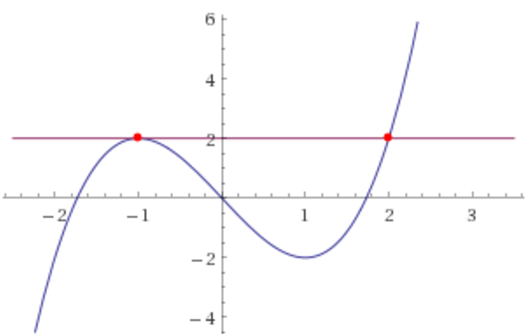
\includegraphics[width=0.4\textwidth]{img-sol/t7-tangent}}
			
			\exer Determina els coeficients $a$ , $b$ i $c$ de la funció $f(x) = ax^{3} + bx + c$, que passa pel punt $A(1, 2)$ i és tangent a la recta $y = x$ en el punt $O(0, 0)$.
			
			\answers{Plantejam un sistema. Ha de passar per $A$: $2=a+b+c$. Ha de passar per $O$: $0=c$. Ha de tenir derivada 1 a $x=0$: $b=1$. Llavors $a=1$, $b=1$, $c=0$}
			
			\exer Determina els coeficients $a$, $b$ i $c$ perquè les funcions $f(x) = x^{3} + bx + c$ i $g(x) = a x - x^{2}$ tinguin la mateixa recta tangent en el punt $A(1, 0)$.
			
			\answers{Plantejam un sistema. Les dues rectes han d'ésser secants a $A$: $0=1+b+c$; $0=a-1$. Ha de tenir igual derivada a $x=1$:  $3+b=a-2$. Llavors $a=1$, $b=-4$, $c=3$}
				
			\exer Determina el coeficient $a$, perquè la funció $f(x) = x^{2} + a$, sigui tangent a la recta $y = x$.
			
			\answers{En algun punt de $f$ el seu pendent ha de valer 1: $2x=1$. Això només passa quan $x=1/2$; $y=1/2$. Llavors, aquest punt ha d'ésser també un punt de la corba: $\frac{1}{2}=\frac{1}{4}+a$, llavors $a=\frac{1}{4}$ }
			
		\end{mylist}
	
	
	
	
		
		\section{Monotonia i  extrems d'una funció}
		
		\begin{theorybox}
			La primera derivada d'una funció ens serveix per saber si és creixent o decreixent, així com determinar els seus màxims i mínims relatius.
			
			\begin{center}
			\begin{tabular}{p{6cm}| p{8cm}}
				Si $f'(x)>0$ & La funció és creixent \\ [0.15cm] \hline
				Si $f'(x)<0$ & La funció és decreixent \\ [0.15cm] \hline 
				Si la funció té un extrem \par (màxim o mínim) & es compleix $f'(x)=0$
			\end{tabular}
			\end{center}
			Les solucions de l'equació $f'(x)=0$ s'anomenen \textbf{punts crítics} i són possibles màxims o mínims.
		\end{theorybox}
		
		
		\begin{mylist}
			
			
			\exer Si $f'(x) = x\cdot (3 - x)$, quina de les següents gràfiques podria ser la de $f (x)$? 
			
			\begin{center}
				\includegraphics*[height=1.1in, keepaspectratio=true]{img-07/chap-deriv-opt-a.pdf} \hspace{0.24cm}
				\includegraphics*[height=1.1in, keepaspectratio=true]{img-07/chap-deriv-opt-b.pdf}  \hspace{0.24cm}
				\includegraphics*[height=1.1in, keepaspectratio=true]{img-07/chap-deriv-opt-c.pdf}  \hspace{0.24cm}
				\includegraphics*[height=1.1in, keepaspectratio=true]{img-07/chap-deriv-opt-d.pdf}   
			\end{center}
		
		\answers{Només pot ésser la d) perquè la derivada s'anul·la en dos punts $x=0$ i $x=3$, llavors són dos punts on la recta tangent és horitzontal.}
		
			\exer Determina els intervals de creixement i decreixement de
		\begin{tasks}(2)
			\task $f (x) = \dfrac{1}{ x^{2}}$.
			\task $f (x) = \dfrac{1}{ x}$.
			\task $f (x) = x^{3} - 3x^{2} + 4$
			\task $f (x) = x^{3} - 6x^{2} + 9x + 6$
		\end{tasks}
		
		\answers{[  Creix $(-\infty,0)$\par Decreix $(0,\infty)$. No té extrems, 
					Sempre decreix, 
					Creix $(-\infty,0)\cup(2,+\infty)$\par Decreix $(0,2)$, 
					Creix $(-\infty,1)\cup(3,+\infty)$\par Decreix $(1,3)$]}
			
		\end{mylist}

		\begin{resolt}{Troba els extrems de
				
				 $y=x^3-3x^2$}
			Calculam la derivada $y'=3x^2-6x$. 
			Resolem l'equació $3x^2-6x=0$ $\rightarrow$ $x=0$ i $x=2$ són els punts singulars.
			\vspace{0.25cm}
			
			Per saber si aquests punts són màxims o mínims estudiam el creixement/decreixement. Per això calculam el signe de $f'$ 
			\vspace{0.35cm}
			
			\begin{center}
			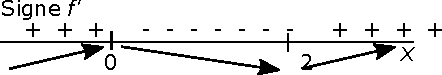
\includegraphics[width=5cm]{img-07/signefprima}
			\end{center}
			\vspace{0.35cm}
			
			La funció és creixent a $(-\infty, 0) \cup (2,+\infty)$ i decreixent a $(0,2)$. Té un màxim al punt $(0,0)$ i un mínim relatiu a $(2,-4)$.
			
		\end{resolt}
	\vspace{0.5cm}
		
		\begin{mylist}
			 
			\exer Determina els intervals de creixement, decreixement, els màxims i mínims de les funcions següents
			\begin{tasks}(2)
				\task $f(x)=x^3-6x^2+9x-8$
				\task $f(x)=\dfrac{x}{\ln x}$
				\task $f(x)=\dfrac{x}{x^2-5x+4}$
				\task $f(x)=x^2 e^x$
				\task $f(x)=\dfrac{x^2}{1+x^2}$
				\task $f(x)=x+5-2\sin x$
			\end{tasks}
		
		\answers{[Creix $(-\infty,1)\cup(3,+\infty)$\par Decreix $(1,3)$.\par Màx: $(1,-4)$ \par Min: $(3,-8)$,
			Creix $(e,+\infty)$\par Decreix $(0,1)\cup(1,e)$.\par  Min: $(e,e)$,
			Creix $(-2,1)\cup(1,2)$\par Decreix $(-\infty,-2)\cup(2,4)\cup(4,+\infty)$.\par Màx: $(2,-1)$ \par Min: $(-2,-1/9)$,
			Creix $(-\infty,-2)\cup(0,+\infty)$\par Decreix $(-2,0)$.\par Màx: $(-2,\frac{4}{e^2})$\par Min: $(0,0)$,
			Creix $(0,+\infty)$\par Decreix $(-\infty,0)$.\par  Min: $(0,0)$,
			Màx: $x=-\frac{\pi}{3}+2\pi n$ \par Min: $x=\frac{\pi}{3}+2\pi n$
			]}
		
		\exer  Determina els intervals de creixement i decreixement de la funció: $y = x^3 - 3x$. Com és en $x = 0$? I en $x = 2$? I en $x = -2$? Repeteix l'activitat per a la funció $y = x^3 + 3x$.
		\answers{La funció $y = x^3 - 3x$ té un màxim a $(-1,2)$ i un mínim $(1,-2)$. A $x=0$ és decreixent. A $x=\pm 2$ és creixent. La funció $y = x^3 + 3x$ és sempre creixent; no té extrems. }
		
			\exer Determina els intervals de creixement i decreixement de  $f (x) = 2x^{3} - 3x^{2} + 3$. Calcula els seus màxims i mínims. Fes un esbós de la seva gràfica.
			
			\answers{Té un màxim a $(0,3)$ i un mínim a $(1,2)$. Gràfica:\par 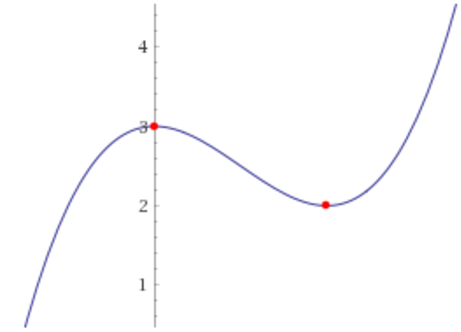
\includegraphics[width=0.4\textwidth]{img-sol/t7-47}}
			
			\exer Determina els intervals de creixement i decreixement de  $f (x) = x^{3} - 9x$. Calcula els seus màxims i mínims. Fes un esbós de la seva gràfica.
			
				\answers{Té un màxim a $(-\sqrt{3},6\sqrt{3})$ i un mínim a $(\sqrt{3},-6\sqrt{3})$. Gràfica:\par 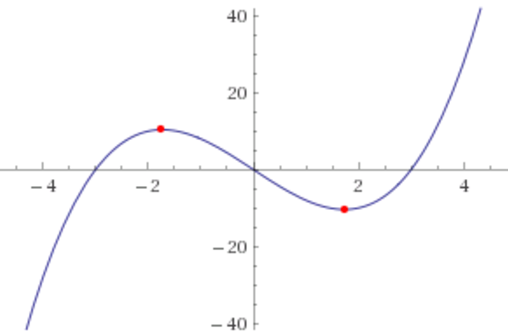
\includegraphics[width=0.4\textwidth]{img-sol/t7-48}}
			
		%	\exer Calcula els màxims i mínims relatius i absoluts de la funció $f(x) = 4x^{3} - 6x^{2} + 72x$ en l'interval [-7, 2] i en l'interval [0, 8].
			
			
		\end{mylist}
	
	
	\section{Curvatura i  punts d'inflexió}
	
	\begin{theorybox}
		\textbf{Derivades successives:}
		
		Donat que la derivada d'una funció és una altra funció, aquesta es pot tornar a derivar obtenint així la derivada segona. Si derivam la derivada segona obtenim la derivada tercera i així successivament.
		
			\begin{minipage}{0.5\textwidth}
		Per exemple, $y=x^4-5x^2-3$
		
		Té derivada primera $y'=4x^3-10x$
		
		Derivada segona $y''=12 x^2 -10$
			\end{minipage}
			\begin{minipage}{0.5\textwidth}
		Derivada tercera $y'''=24 x$
		
		Derivada quarta $y^{iv}=24$
		
		i  les demés derivades són zero.
			\end{minipage}
	\end{theorybox}

\begin{mylist}
	\begin{noexerbreak}
		
	\exer Calcula la derivada segona de les següents funcions
	\begin{tasks}(2)
		\task $f(x)=x^3-3x^2+x-2$
		\task $f(x)=\sin x + \ln x$
		\task $f(x)=\dfrac{1}{1+x^2}$
		\task $f(x)=x\cdot \ln x$
		\task $f(x)=\dfrac{x+1}{x-1}$
		\task $f(x)=x^2-3\cos x^2$
	\end{tasks}

	\answers{[$y''=6x-6$, $y''=-\sin x -\frac{1}{x^2}$, $y''=\dfrac{6x^2-2}{(x^2+1)^3}$, $y''=\dfrac{1}{x}$, $y''=\dfrac{4}{(x-1)^3}$, $y''=6\sin x^2 + 12 x^2 \cos x^2 + 2$]}

	\end{noexerbreak}
\end{mylist}

	\begin{theorybox}
			\begin{minipage}{0.4\textwidth}
				\includegraphics*[width=\textwidth]{img-07/curvatura.png}
			\end{minipage}
			\begin{minipage}{0.6\textwidth}
				\begin{itemize}
					\item Una funció és \textbf{convexa} si la recta tangent es troba per damunt d'ella.
					\item Una funció és \textbf{còncava} si la recta tangent es troba per davall d'ella.
					\item Una funció té un \textbf{punt d'inflexió} si la recta tangent l'atravessa.
				\end{itemize}
			\end{minipage}
	\end{theorybox}
	
	
	\begin{theorybox}
	  La segona derivada d'una funció ens serveix per determinar la seva curvatura i els punts d'inflexió.
	 
	 \begin{center}
	 	\begin{tabular}{p{6cm}| p{8cm}}
	 		Si $f''(x)>0$ & La funció és còncava $\cup$ \\ [0.15cm] \hline
	 		Si $f''(x)<0$ & La funció és convexa $\cap$ \\ [0.15cm] \hline 
	 		Si la funció té un punt d'inflexió  & es compleix $f''(x)=0$
	 	\end{tabular}
	 \end{center}
	 
	 A més, existeix una condició entre els extrems i la segona derivada:
	 \begin{center}
	 	\begin{tabular}{p{6cm}| p{8cm}}
	 		Si $f'(a)=0$ i $f''(a)>0$ & $x=a$ és un mínim relatiu \\ [0.15cm] \hline
	 		Si $f'(a)=0$ i $f''(a)<0$ & $x=a$ és un màxim relatiu  \\ [0.15cm] 
	 	\end{tabular}
	 \end{center} 
	\end{theorybox}
	
	
	\begin{mylist}
	
		\exer Determina la curvatura i els punts d'inflexió de les funcions següents
		\begin{tasks}(2)
			\task $f(x)=x^3-3x+2$
			\task $f(x)=x^4-6x^2+4$
			\task $f(x)=\dfrac{1}{x}$
			\task $f(x)=\dfrac{1}{1+x^2}$
			\task $f(x)=\dfrac{x}{1+x^2}$
			\task $f(x)=e^{-2x^2}$
		\end{tasks}
	
	\answers{[$y''=6x$\par Còncava: $(0,+\infty)$  \par Convexa: $(-\infty,0)$ \par P.I. $(0,2)$,
			$y''=12x^2-12$\par Còncava: $(-\infty,-1)\cup(1,+\infty)$  \par Convexa: $(-1,1)$ \par P.I. $(\pm 1,-1)$,  
			$y''=\frac{2}{x^3}$\par Còncava: $(0,+\infty)$  \par Convexa: $(-\infty,0)$ \par P.I. no en té,  
			$y''=\dfrac{6x^2-2}{(x^2+1)^3}$\par Còncava: $(-\infty,-\sqrt{3}/3)\cup(\sqrt{3}/3,+\infty)$  \par Convexa: $(-\sqrt{3}/3,\sqrt{3}/3)$ \par P.I. $x=\pm\sqrt{3}/3$, 
			$y''=\dfrac{2x(x^2-3)}{(x^2+1)^3}$\par Còncava: $(-\sqrt{3},0)\cup(\sqrt{3},+\infty)$  \par Convexa: $(-\infty,-\sqrt{3})\cup(0,\sqrt{3})$ \par P.I. $(0,0)$; $(\pm \sqrt{3},\pm \sqrt{3}/4)$,   
			$y''=4e^{-2x^2}(4x^2-1)$\par Còncava: $(-\infty,-1/2)\cup(1/2,+\infty)$  \par Convexa: $(-1/2,1/2)$ \par P.I. $x=\pm\frac{1}{2}$]}
	\end{mylist}
 
   
 \section{Representació de funcions}
 
 
	\begin{center}
		\textbf{\footnotesize Taula resum per a la representació de corbes $y=f(x)$}
		\setlength\LTleft{0pt}
		\setlength\LTright{0pt}
		\fontsize{10.5}{11}
		\def\arraystretch{1}
		\begin{longtable}[!htb]{|p{0.4\textwidth}|p{0.57\textwidth}|}
			\hline
			1. \textbf{Domini}, $Dom\, f$ & Conjunt de valors de $x$ pels quals hi ha gràfica. \\  [1.5ex] \hline 
			2.  \textbf{Continuïtat} & Valors del $Dom\, f$ on és contínua. \\  [1.5ex] \hline 
			3.  \textbf{Periodicitat} & Si escau, determinar el període $T$; el valor mínim pel qual $f(x)=f(x+T)$. \\  [1.5ex] \hline 
			4.  \textbf{Simetries}
			
			$f$ parell $\rightarrow$ Simetria respecte l'eix OY
			
			$f$ senar $\rightarrow$ Simetria respecte l'origen 
			
			& Cacularem l'expressió de $f(-x)$:
			
			Si $f(-x)=f(x)$ té simetria parell
			
			Si $f(-x)=-f(x)$ té simetria senar
			\\  [1.5ex] \hline 
			5. \textbf{Asímptotes}
			
			Verticals: $x=a$
			
			Horitzontals: $y=n$
			
			Obliqües: $y=mx+n$
			
			& 
			\newline
			$\limx{a} f(x)=\pm \infty$
			
			$n=\limx{\infty} f(x)$
			
			$m=\limx{\infty} \frac{f(x)}{x}$; \quad $n=\limx{\infty} \left(f(x)-mx\right)$
			
			
			Calculam la posició relativa de la corba respecte les asímptotes.
			\\  [1.5ex] \hline 
			6. \textbf{Punts de tall amb els eixos}
			
			Eix OX
			
			Eix OY
			
			Regions o signe
			& \newline
			Solucions de $f(x)=0$. Pot haver-hi 0, 1 o uns quants
			
			Punt $(0, f(0))$. Pot haver-hi 0 o 1
			
			$f(x)<0$, $f(x)>0$  
			\\  [1.5ex] \hline 
			7. \textbf{Màxims i mínims relatius}
			\newline
			\newline
			\newline
			
			\textbf{Creixement i decreixement}
			
			& Punts crítics. Resolem $f'(x)=0$
			
			$f''(a)<0$ $\rightarrow$ $x=a$ un màxim relatiu
			
			$f''(a)>0$ $\rightarrow$ $x=a$ un mínim relatiu
			\newline
			
			$f'(a)<0$ $\rightarrow$ $f$ decreixent en $x=a$
			
			$f'(a)>0$ $\rightarrow$ $f$ creixent en $x=a$
			\\  [1.5ex] \hline 
			8. \textbf{Punts d'inflexió}
			\newline
			
			
			\textbf{Curvatura}
			
			& Resolem $f''(x)=0$ i comprovam $f'''(x)\neq 0$
			\newline
			
			$f''(a)<0$ $\rightarrow$ $f$ Convexa $\cap$ en $x=a$
			
			$f''(a)>0$ $\rightarrow$ $f$ Còncava $\cup$ en $x=a$
			\\  [1.5ex] \hline 
			9. \textbf{Gràfica} & Fer el dibuix a partir de la informació anterior \\  [1.5ex] \hline 
		\end{longtable}
	\end{center}





 \pagebreak
\begin{center}
	\setlength\LTleft{0pt}
	\setlength\LTright{0pt}
	\fontsize{10.5}{11}
	\def\arraystretch{1.01}
	\begin{longtable}[h]{|p{0.3\textwidth}|p{0.35\textwidth}|p{0.3\textwidth}|}
		\hline
		\multicolumn{3}{|c|} { 
			\cellcolor{lightgray} \textbf{Representació de $f(x)=x^3-3x+2$} }
		\\  [1.5ex] \hline 
		1. \textbf{Domini} & $(-\infty, +\infty)$ & Tipus: Polinòmica  \\  [1.5ex] \hline 
		2. \textbf{Simetries} & \multicolumn{2}{l|}{No en té} \\  [1.5ex] \hline 
		3. \textbf{Talls amb els eixos}
		
		Talls amb l'eix OX:
		
		Tall amb l'eix OY: & \multicolumn{2}{p{10cm}|}{
			
			$(x=-2, y=0)$  i $(x=1, y=0)$ 
			\par
			
			$(x=0, y=2)$} \\  [1.5ex] \hline
		
		4. \textbf{Asímptotes} & & \\  [1.5ex] \hline 
		Verticals: & No en té & \\  [1.5ex] \hline 
		Horitzontals: &No en té & \\  [1.5ex] \hline 
		Obliqües: &No en té & \\  [1.5ex] \hline   	
		Branques: & $\limx{-\infty} f(x)=-\infty$ & $\limx{+\infty} f(x)=+\infty$ \\  [1.5ex] \hline    
		5. \textbf{Derivada primera} & \multicolumn{2}{l|} {$f'(x)=3x^2-3$} \\  [1.5ex] \hline 
		\textbf{Solucions de} $f'(x)=0$ & \multicolumn{2}{l|} {$x=-1$, $x=1$} \\  [1.5ex] \hline 
		6.  \textbf{Creixement}: & Creixent $(-\infty,-1)\cup(1,+\infty)$ & Decreixent $(-1,1)$  \\  [1.5ex] \hline  
		7. \textbf{Extrems} & Màxim $(x=-1, y=4)$ & Mínim $(x=1, y=0)$ \\  [1.5ex] \hline 
		8. \textbf{Derivada segona} & \multicolumn{2}{l|} {$f''(x)=6x$} \\  [1.5ex] \hline 
		\textbf{Solucions de $f''(x)=0$} & \multicolumn{2}{l|} {$x=0$} \\  [1.5ex] \hline 
		9.  \textbf{Curvatura}: & Còncava $(0, + \infty)$ & Convexa $(-\infty,0)$  \\  [1.5ex] \hline   
		10. \textbf{Punts d'inflexió} & \multicolumn{2}{l|} {$(x=0, y=2)$} \\  [1.5ex] \hline 
		\multicolumn{3}{|p{\textwidth}|} {\textbf{Gràfica}: 
			
			\begin{center}
				\includegraphics*[width=0.9\textwidth]{img-07/chap-deriv-polinomica1.pdf}
			\end{center}
		}
		\\  [1.5ex] \hline 
	\end{longtable}
\end{center}
\pagebreak

\begin{center}
	\setlength\LTleft{0pt}
	\setlength\LTright{0pt}
	\fontsize{10.5}{11}
	\def\arraystretch{1.01}
	\begin{longtable}[h]{|p{0.3\textwidth}|p{0.35\textwidth}|p{0.3\textwidth}|}
		\hline
		\multicolumn{3}{|c|} { 
			\cellcolor{lightgray} \textbf{Representació de $f(x)=x^4-2x^2-8$} }
		\\  [1.5ex] \hline 
		1. \textbf{Domini} & $(-\infty, +\infty)$ & Tipus: Polinòmica \par  (biquadrada) \\  [1.5ex] \hline 
		2. \textbf{Simetries} & \multicolumn{2}{l|}{$f(-x)=f(x)$ simètrica parell} \\  [1.5ex] \hline 
		3. \textbf{Talls amb els eixos}
		
		Talls amb l'eix OX:
		
		Tall amb l'eix OY: & \multicolumn{2}{p{10cm}|}{
			
			$(x=-2, y=0)$; $(x=2, y=0)$ 
			\par
			
			$(x=0, y=-8)$} \\  [1.5ex] \hline
		
		4. \textbf{Asímptotes} & & \\  [1.5ex] \hline 
		Verticals: & No en té & \\  [1.5ex] \hline 
		Horitzontals: &No en té & \\  [1.5ex] \hline 
		Obliqües: &No en té & \\  [1.5ex] \hline   	
		Branques: & $\limx{-\infty} f(x)=+\infty$ & $\limx{+\infty} f(x)=+\infty$ \\  [1.5ex] \hline    
		5. \textbf{Derivada primera} & \multicolumn{2}{l|} {$f'(x)=4x^3-4x$} \\  [1.5ex] \hline 
		\textbf{Solucions de} $f'(x)=0$ & \multicolumn{2}{l|} {$x=-1$, $x=0$, $x=1$} \\  [1.5ex] \hline 
		6.  \textbf{Creixement}: & Creixent $(-1,0)\cup(1,+\infty)$ & Decreixent $(-\infty,-1)\cup(0,1)$  \\  [1.5ex] \hline  
		7. \textbf{Extrems} & Màxim $(x=0, y=-8)$ & Mínims $(x=-1, y=-9)$, $(x=1, y=-9)$ \\  [1.5ex] \hline 
		8. \textbf{Derivada segona} & \multicolumn{2}{l|} {$f''(x)=12x^2-4$} \\  [1.5ex] \hline 
		\textbf{Solucions de $f''(x)=0$} & \multicolumn{2}{l|} {$x=-{\sqrt{3} \over 3}$, $x={\sqrt{3} \over 3}$} \\  [1.5ex] \hline 
		9.  \textbf{Curvatura}: & Còncava $(-\infty, -\sqrt{3}/3) \cup (\sqrt{3}/3,+\infty)$ & Convexa $(-\sqrt{3}/3, \sqrt{3}/3)$  \\  [1.5ex] \hline   
		10. \textbf{Punts d'inflexió} & \multicolumn{2}{l|} {$(x=-\sqrt{3}/3, y=-8.56)$, $(x=\sqrt{3}/3, y=-8.56)$} \\  [1.5ex] \hline 
		\multicolumn{3}{|p{\textwidth}|} {\textbf{Gràfica}: 
			
			\begin{center}
				\includegraphics*[width=0.9\textwidth]{img-07/chap-deriv-polinomica2.pdf}
			\end{center}
		}
		\\  [1.5ex] \hline 
	\end{longtable}
\end{center}
\pagebreak


\begin{center}
	\setlength\LTleft{0pt}
	\setlength\LTright{0pt}
	\fontsize{10.5}{11}
	\def\arraystretch{1.01}
	\begin{longtable}[h]{|p{0.3\textwidth}|p{0.35\textwidth}|p{0.3\textwidth}|}
		\hline
		\multicolumn{3}{|c|} { 
			\cellcolor{lightgray} \textbf{Representació de $f(x)=\dfrac{x^2-4}{x^2+4}$} }
		\\  [1.5ex] \hline 
		1. \textbf{Domini} & $(-\infty, +\infty)$ & Tipus: Racional  \\  [1.5ex] \hline 
		2. \textbf{Simetries} & \multicolumn{2}{l|}{Simètrica parell $f(-x)=f(x)$} \\  [1.5ex] \hline 
		3. \textbf{Talls amb els eixos}
		
		Talls amb l'eix OX:
		
		Tall amb l'eix OY: & \multicolumn{2}{p{10cm}|}{
			
			$(x=-2, y=0)$  i $(x=2, y=0)$ 
			\par
			
			$(x=0, y=-1)$} \\  [1.5ex] \hline
		
		4. \textbf{Asímptotes} & & \\  [1.5ex] \hline 
		Verticals: & No en té & \\  [1.5ex] \hline 
		Horitzontals: & $y=1$ & $\limx{\infty} f(x)=1$ per davall  \\  [1.5ex] \hline 
		Obliqües: &No en té & \\  [1.5ex] \hline   	
		Branques: &No en té &   \\  [1.5ex] \hline    
		5. \textbf{Derivada primera} & \multicolumn{2}{l|} {$f'(x)=\dfrac{16x}{(x^2+4)^2}$} \\  [1.5ex] \hline 
		\textbf{Solucions de} $f'(x)=0$ & \multicolumn{2}{l|} {$x=0$} \\  [1.5ex] \hline 
		6.  \textbf{Creixement}: & Creixent $(0,+\infty)$ & Decreixent $(-\infty,0)$  \\  [1.5ex] \hline  
		7. \textbf{Extrems} & Màxim no en té & Mínim $(x=0, y=-1)$ \\  [1.5ex] \hline 
		8. \textbf{Derivada segona} & \multicolumn{2}{l|} {$f''(x)=\dfrac{64-48x^2}{(x^2+4)^3}$} \\  [1.5ex] \hline 
		\textbf{Solucions de $f''(x)=0$} & \multicolumn{2}{l|} {$x\approx -1.15$, $x\approx +1.15$} \\  [1.5ex] \hline 
		9.  \textbf{Curvatura}: & Còncava $(-1.15, 1.15)$ & Convexa 
		
		$(-\infty, -1.15) \cup (1.15, +\infty)$  \\  [1.5ex] \hline   
		10. \textbf{Punts d'inflexió} & \multicolumn{2}{l|} {$(x=-1.15, y=-0.5)$, $(x=1.15, y=-0.5)$} \\  [1.5ex] \hline 
		\multicolumn{3}{|p{\textwidth}|} {\textbf{Gràfica}: 
			
			\begin{center}
				\includegraphics*[width=0.9\textwidth]{img-07/chap-deriv-racional1.pdf}
			\end{center}
		}
		\\  [1.5ex] \hline 
	\end{longtable}
\end{center}
\pagebreak

\begin{center}
	\setlength\LTleft{0pt}
	\setlength\LTright{0pt}
	\fontsize{10.5}{11}
	\def\arraystretch{1.01}
	\begin{longtable}[h]{|p{0.3\textwidth}|p{0.35\textwidth}|p{0.3\textwidth}|}
		\hline
		\multicolumn{3}{|c|} { 
			\cellcolor{lightgray} \textbf{Representació de $f(x)=\dfrac{x^2+3}{x-1}$} }
		\\  [1.5ex] \hline 
		1. \textbf{Domini} & $\mathbb{R}-\{1\}$ & Tipus: Racional  \\  [1.5ex] \hline 
		2. \textbf{Simetries} & \multicolumn{2}{l|}{No té simetria} \\  [1.5ex] \hline 
		3. \textbf{Talls amb els eixos}
		
		Talls amb l'eix OX:
		
		Tall amb l'eix OY: & \multicolumn{2}{p{10cm}|}{
			
			No hi talla 
			\par
			
			$(x=0, y=-3)$} \\  [1.5ex] \hline
		
		4. \textbf{Asímptotes} & & \\  [1.5ex] \hline 
		Verticals: & $x=1$ &  $\limx{1^-} f(x)=-\infty$, \par $\limx{1^+} f(x)=+\infty$  \\ [1.5ex] \hline 
		Horitzontals: & No en té &  \\  [1.5ex] \hline 
		Obliqües: & $y=x+1$ & $x\rightarrow -\infty$ per davall,\par $x\rightarrow +\infty$ per damunt  \\ [1.5ex] \hline   	
		
		5. \textbf{Derivada primera} & \multicolumn{2}{l|} {$f'(x)=\dfrac{x^2-2x-3}{(x-1)^2}$} \\  [1.5ex] \hline 
		\textbf{Solucions de} $f'(x)=0$ & \multicolumn{2}{l|} {$x=-1$, $x=3$} \\  [1.5ex] \hline 
		6.  \textbf{Creixement}: & Creixent 
		$(-\infty,-1)\cup (3,+\infty)$ & Decreixent $(-1,1)\cup (1,3)$  \\  [1.5ex] \hline  
		7. \textbf{Extrems} & Mínim $(x=3,y=6)$ & Màxim $(x=-1, y=-2)$ \\  [1.5ex] \hline 
		8. \textbf{Derivada segona} & \multicolumn{2}{l|} {$f''(x)=\dfrac{8}{(x-1)^3}$} \\  [1.5ex] \hline 
		\textbf{Solucions de $f''(x)=0$} & \multicolumn{2}{l|} {No en té} \\  [1.5ex] \hline 
		9.  \textbf{Curvatura}: & Còncava $(1,+\infty)$ & Convexa 
		$(-\infty, 1) $  \\  [1.5ex] \hline   
		10. \textbf{Punts d'inflexió} & \multicolumn{2}{l|} {No en té} \\  [1.5ex] \hline 
		\multicolumn{3}{|p{\textwidth}|} {\textbf{Gràfica}: 
			
			\begin{center}
				\includegraphics*[width=0.9\textwidth]{img-07/chap-deriv-racional2.pdf}
			\end{center}
		}
		\\  [1.5ex] \hline 
	\end{longtable}
\end{center}
\pagebreak

\begin{mylist}
	\exer Representa gràficament les següents funcions polinòmiques:
	\begin{tasks}(3)
		\task $y=x(x+2)(x-2)$
		\task $y=x^4-2x^2$
		\task $y=2x^3+5x^2-4x$
		\task $y=-\dfrac{x^3}{6}+x$
		\task $y=x^3-2x^2+x-1$
		\task $y=(x+1)^2 (x-2)$
	\end{tasks}

\answers{[\mbox{}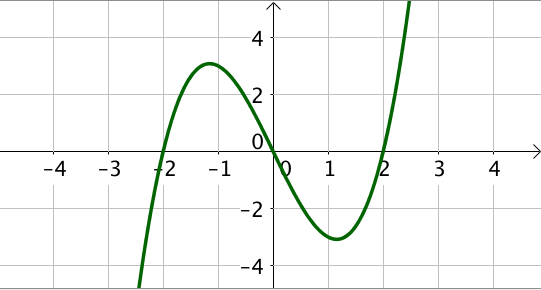
\includegraphics[width=0.4\textwidth]{img-sol/t7-52a}\par
				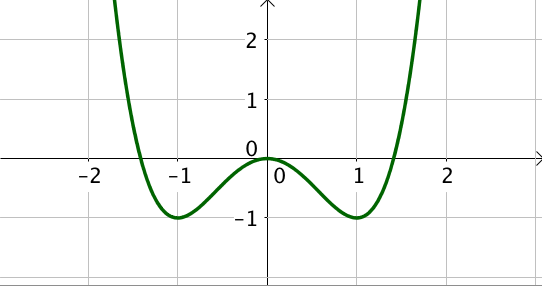
\includegraphics[width=0.4\textwidth]{img-sol/t7-52b}\par
				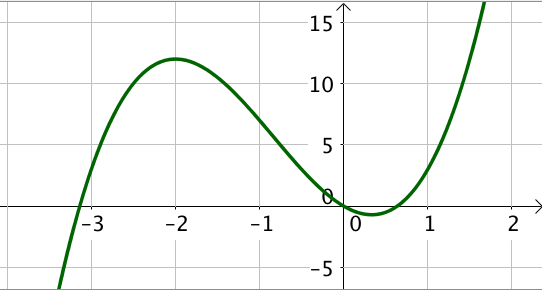
\includegraphics[width=0.4\textwidth]{img-sol/t7-52c}\par
				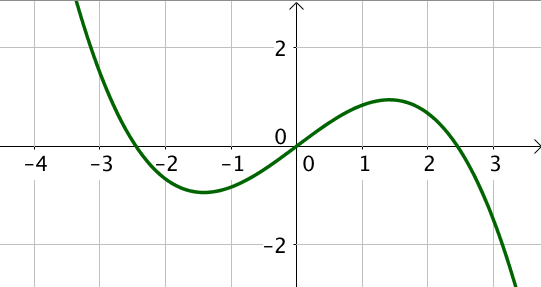
\includegraphics[width=0.4\textwidth]{img-sol/t7-52d}\par
				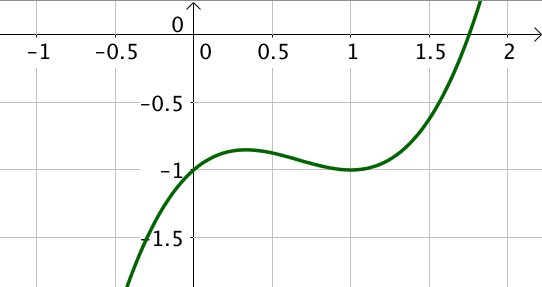
\includegraphics[width=0.4\textwidth]{img-sol/t7-52e}\par
				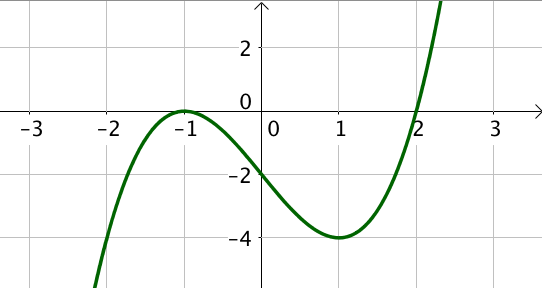
\includegraphics[width=0.4\textwidth]{img-sol/t7-52f}\par]}
	
\addanswersline[cols=1]{}{0}{[Màx $(-1.155,3.079)$; Mín. $(1.1547,-3.079)$, 
	Màx $(0,0)$; Mín. $(-1,-1)$ i $(1,-1)$,  
	Màx $(-2,12)$; Mín. $(\frac{1/3}{3},-\frac{19}{27})$,  
	Màx $(\sqrt{2},\frac{2\sqrt{2}}{3})$; Mín. $(-\sqrt{2},-\frac{2\sqrt{2}}{3})$,
	Màx $(\frac{1}{3},-\frac{23}{27})$; Mín. $(1,-1)$, 
	Màx $(-1,0)$; Mín. $(1,-4)$]}
	
	\exer Representa gràficament les següents funcions racionals:
	\begin{tasks}(3)
		\task $y=\dfrac{x^2-3x+2}{x^2+3x+2}$
		\task $y=\dfrac{4}{x^2-4}$
		\task $y=\dfrac{x^3}{(x-1)^2}$
		\task $y=\dfrac{x^2}{2-x}$
		\task $y=\dfrac{(x-1)^2}{(x+1)^3}$
		\task $y=\dfrac{2x}{x^2+2}$
	\end{tasks}

\answers{[\mbox{}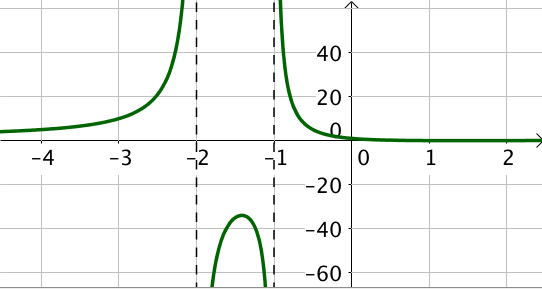
\includegraphics[width=0.4\textwidth]{img-sol/t7-53a}\par
	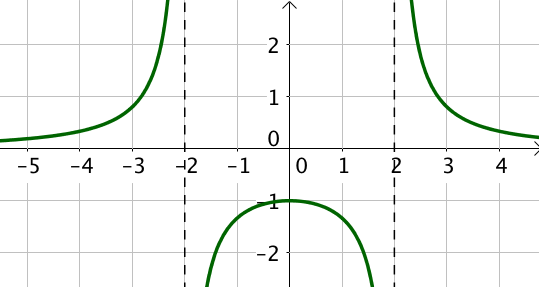
\includegraphics[width=0.4\textwidth]{img-sol/t7-53b}\par
	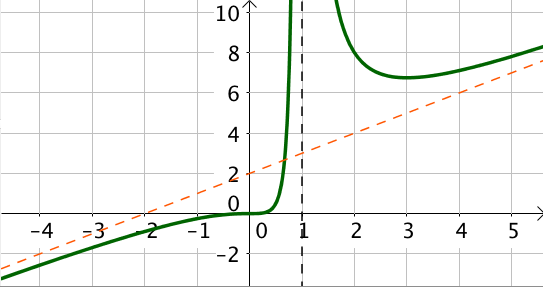
\includegraphics[width=0.4\textwidth]{img-sol/t7-53c}\par
	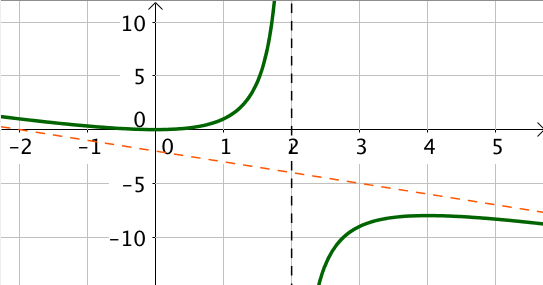
\includegraphics[width=0.4\textwidth]{img-sol/t7-53d}\par
	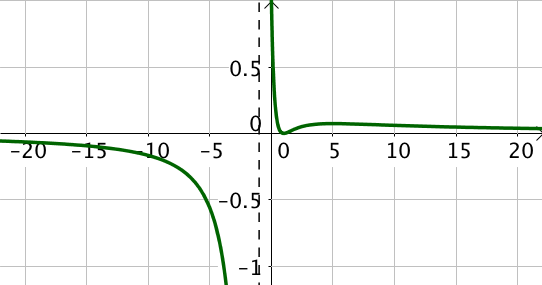
\includegraphics[width=0.4\textwidth]{img-sol/t7-53e}\par
	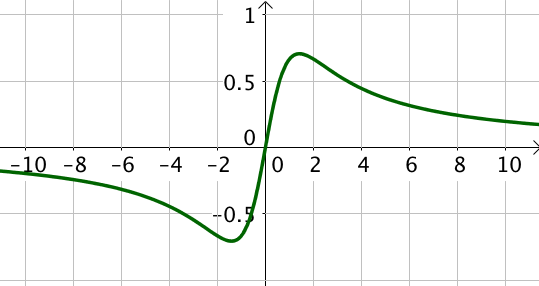
\includegraphics[width=0.4\textwidth]{img-sol/t7-53f}\par]}

\addanswersline[cols=1]{}{0}{[Màx $(-1.414,-33.97)$; Mín. $(1.414,-0.029)$, 
	Màx. no en té; Mín. $(0,-1)$, 
	Màx. no en té; Mín. $(3,\frac{27}{4})$, 
	Màx $(4,-8)$; Mín. $(0,0)$, 
	Màx $(5,\frac{2}{27})$; Mín. $(1,0)$, 
	Màx $(\sqrt{2},\frac{1}{\sqrt{2}})$; Mín. $(-\sqrt{2},-\frac{1}{\sqrt{2}})$
	]}
	
\exer Representa gràficament les següents funcions:
	\begin{tasks}(3)
		\task $y=(x-2) e^x$
		\task $y=2x^2 e^{-x}$
		\task $y=\dfrac{x}{\ln x}$
	\end{tasks}
	
	\answers{[\mbox{}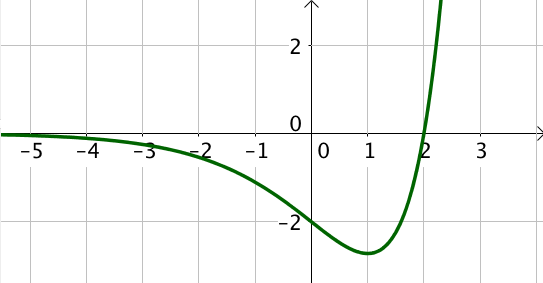
\includegraphics[width=0.4\textwidth]{img-sol/t7-54a}\par
		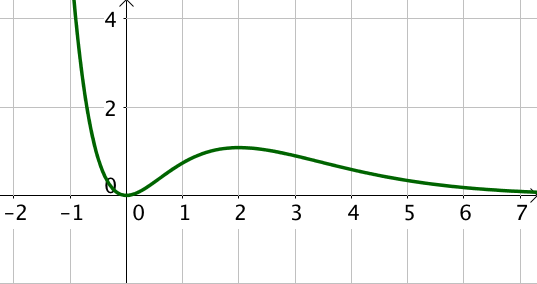
\includegraphics[width=0.4\textwidth]{img-sol/t7-54b}\par
		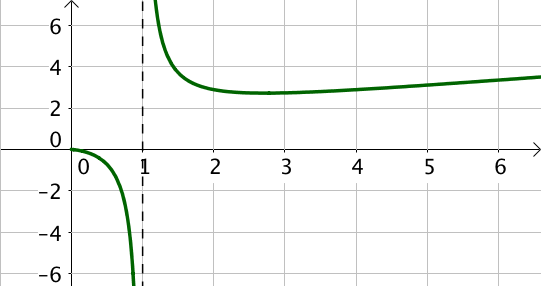
\includegraphics[width=0.4\textwidth]{img-sol/t7-54c}\par]}
	
	\addanswersline[cols=1]{}{0}{[Màx. no en té; Mín. $(1,-e)$, 
		Màx $(2,8/e^2)$; Mín. $(0,0)$, 
		Màx. no en té; Mín. $(e,e)$ 
		]}
	
\end{mylist}

 


\section{Problemes d'optimització}


\begin{theorybox}
	Fins ara t'han donat l'expressió d'una funció $y=f(x)$ i has estat capaç de calcular-ne els màxims i mínims a través de la derivada.\vspace{0.25cm}
	
	Un problema d'optimització és en essència una situació similar, amb una diferència, ara la funció $y=f(x)$ no te la donen; l'hauràs de construir tú a partir d'un enunciat.
\end{theorybox}

\begin{resolt}[E]{
	Expressa el nombre 60 com la suma de dos nombres tals que el seu producte sigui màxim.
}

	Si el primer nombre l'anomenam $x$, el segon nombre serà $60-x$. Ens interessa maximitzar la funció producte:
	$P(x) = x\cdot (60-x) = 60 x - x^2$. Aquesta és la funció que hem d'estudiar.\vspace{0.25cm}
	
	Calculam la derivada $P'(x)= 60 - 2x=0$ i trobam $x=30$. Com que $P''(x)=-2$ és negatiu	
	i concluïm que $x=30$ és un màxim de la funció. Llavors, la solució òptima és $60 = 30 + 30$.
	
\end{resolt}

\begin{mylist}
	
	\exer[-1] Descomposau el nombre 44 en dos sumands tals que el quíntuple del quadrat del primer més el sèxtuple del quadrat del segon sigui mínim.
	\answers{Minimitzeu la funció $f(x)=5x^2+6(44-x)^2$. Trobareu $x=22$.}
	
	\begin{minipage}{0.7\textwidth}			
		\exer[-1] Volem construir caixes usant cartolines rectangulars de 20 cm $\times$ 25 cm. Per a això es talla en cada cantonada un quadrat de costat $x$, i es doblega. Quin valor ha de tenir el costat del quadrat, $x$, retallat perquè les caixes continguin un volum màxim? 
	\end{minipage}
	\begin{minipage}{0.3\textwidth}
		\includegraphics*[width=0.7\textwidth]{img-07/chap-deriv-caixa.pdf}	
	\end{minipage}
	\answers{El volum de les caixes en funció de $x$ és $V(x)=(25-2x)\cdot(20-2x)\cdot x$. El valor pel qual hi ha el màxim és $x=3.68$ cm,
	 $V=820.53$ cm$^{3}$.}
	
	
	\exer Uns barrils per emmagatzemar oli són cilíndrics i tenen una capacitat de 150 litres. Si es desitja construir-los de manera que la seva superfície total sigui mínima, quant ha de mesurar la seva altura i el radi de la seva base?
	
	\answers{$V=\pi r^2 h = 150$ si les mides són $l=\sqrt[3]{dm^3}$, $h=\dfrac{150}{\pi r^2}$. L'àrea total és $S=2\pi r^2 + 2\pi r h = 2 \pi \left( r^2 + \dfrac{150}{\pi r} \right)$. Cercam extrems $S'(r)=0$  $\rightarrow$ $r=\sqrt[3]{\dfrac{75}{\pi}}=2.88$ dm; i l'altura $h=\dfrac{75}{\sqrt[3]{45\pi}}=5.76$ dm.}
	
	\addanswersline[only=tb]{}{0}{
	\newpage

	\heading{Exemples de problemes d'optimització}
	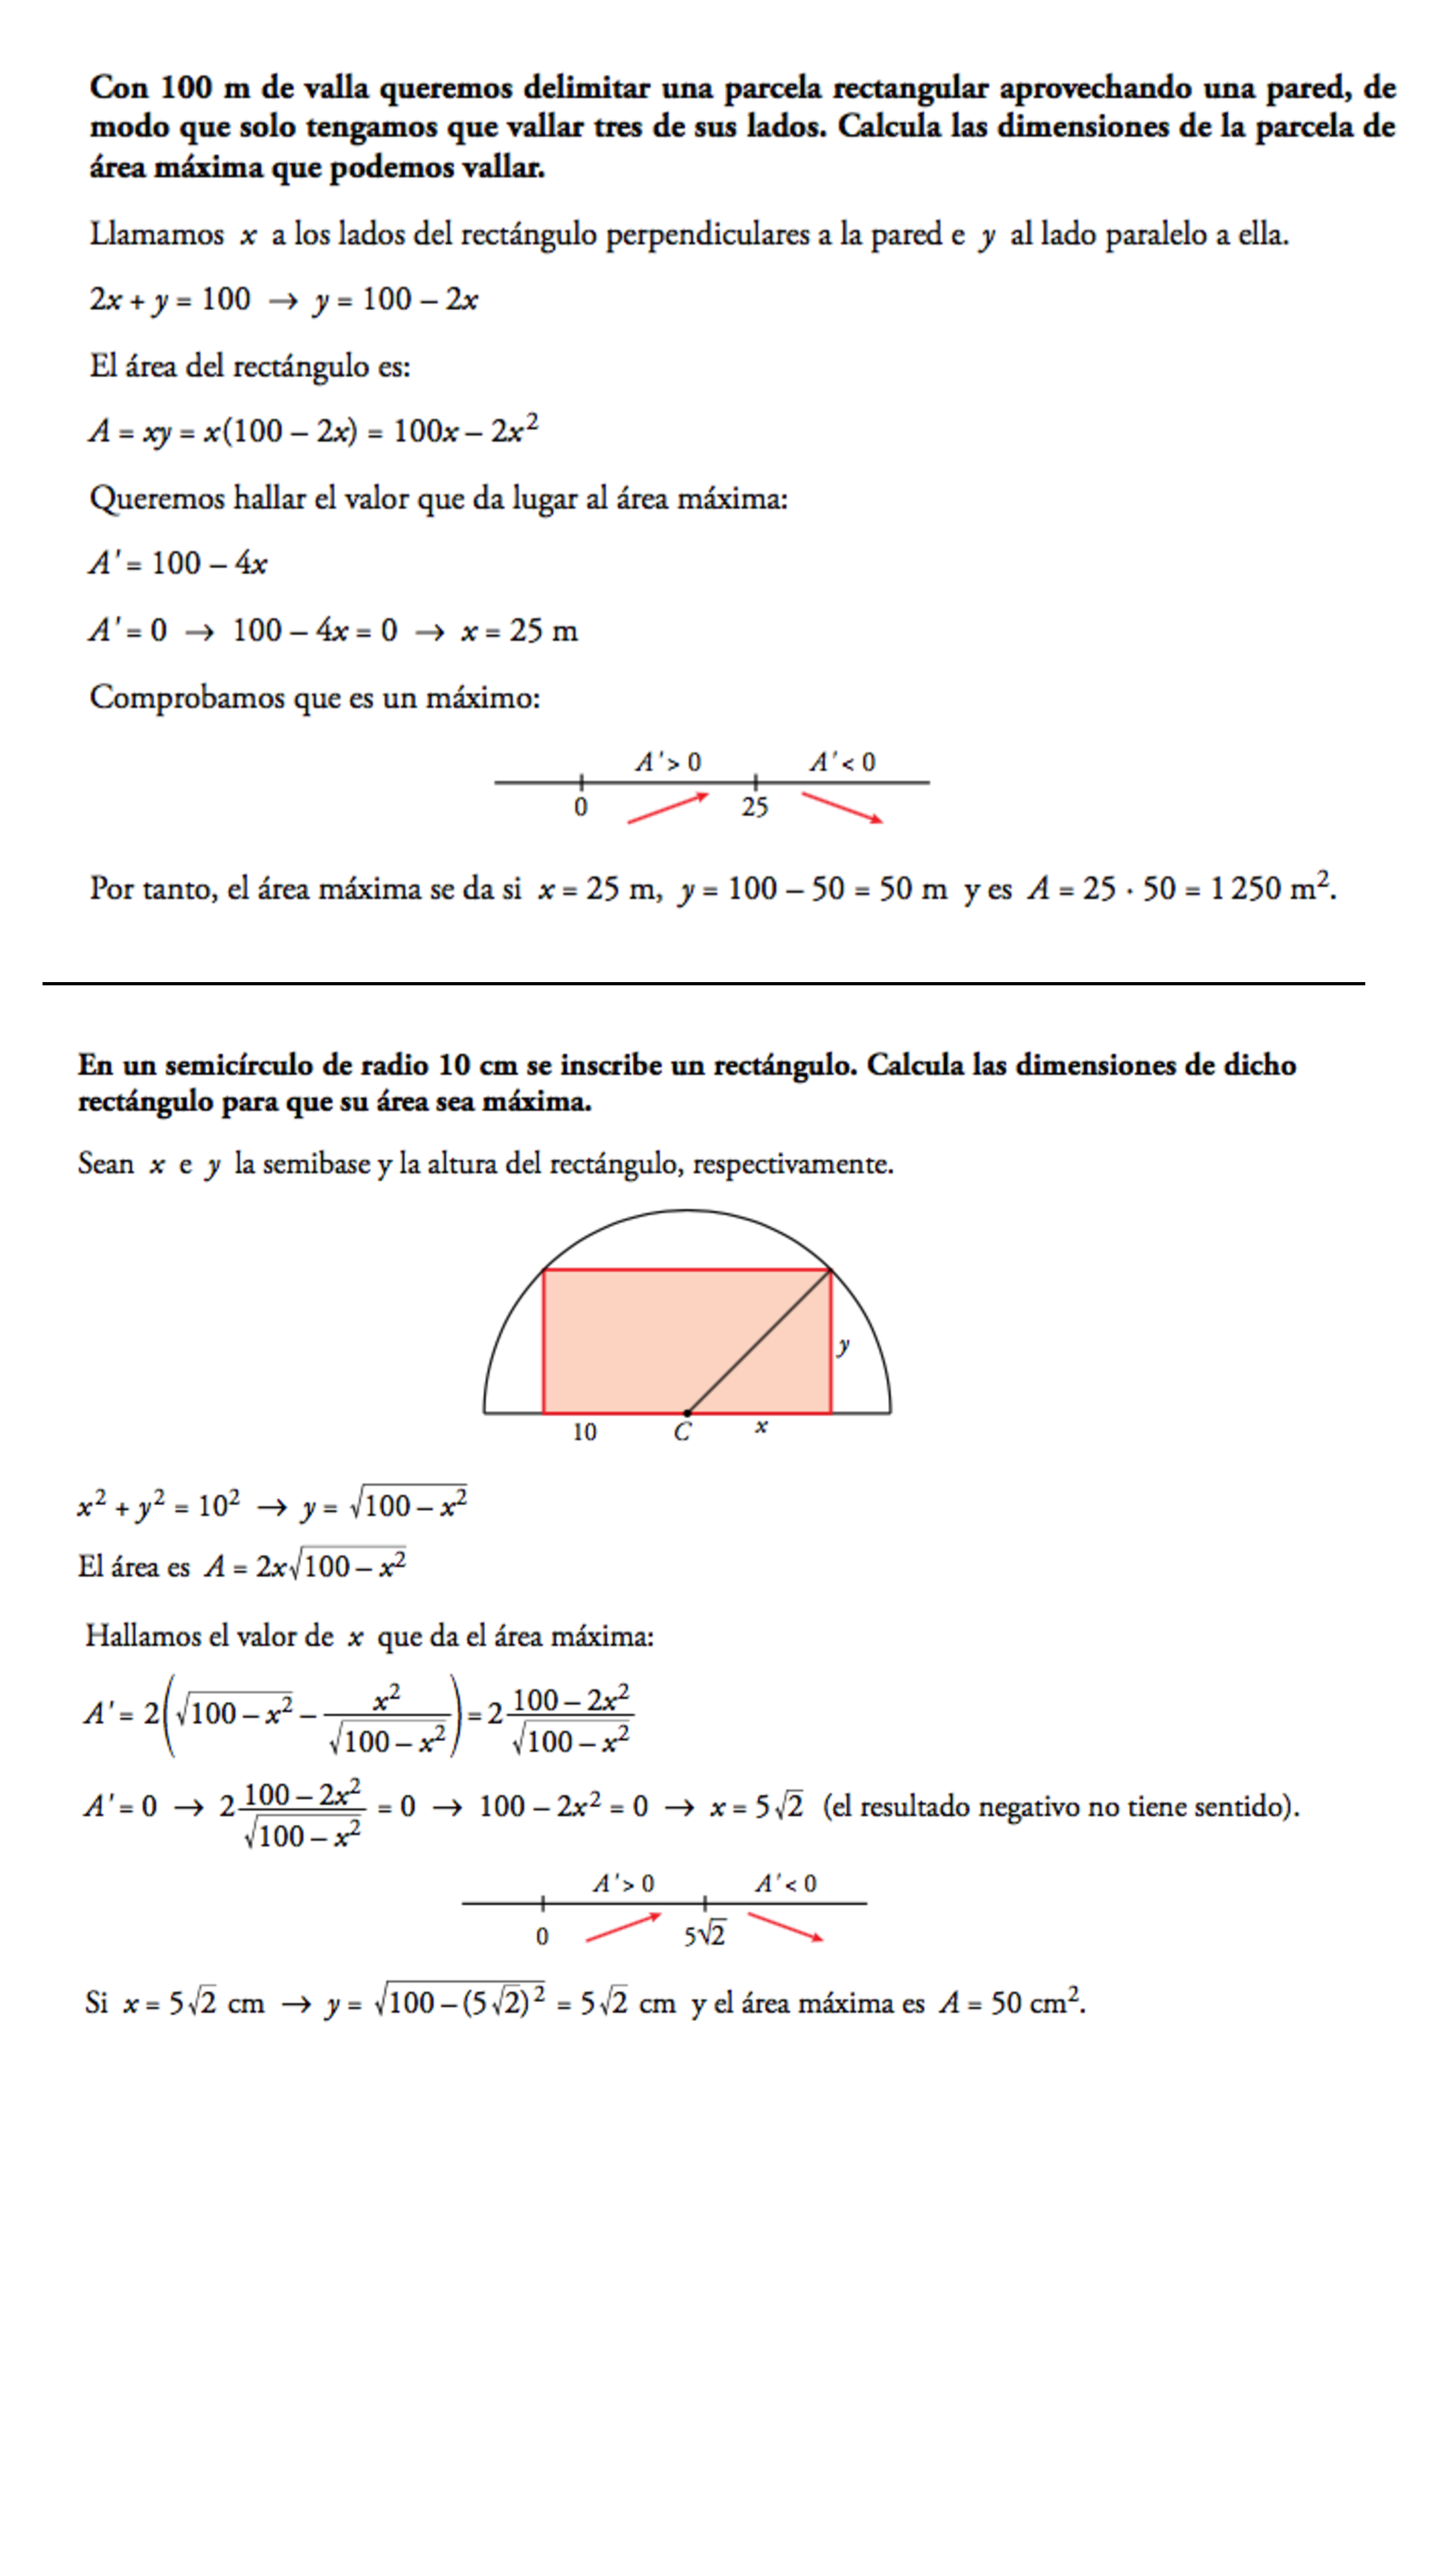
\includegraphics[width=\textwidth]{img-sol/p99-extra}
	}
	
	\exer En fer les proves d'un nou medicament es comprova que segons la dosi, $x$, en mil·ligrams, que s'administri, el percentatge de curacions, i, ve donada per: $y = 100 - \frac{80}{x + 5}$. No obstant això el medicament té efectes secundaris ja que perjudica al ronyó. El nombre de malalts als quals el tractament produeix efectes secundaris augmenta un 2\% per cada mil·ligram que s'augmenta la dosi. Podries ajudar a determinar la dosi de medicament adequada? Raona la resposta.
	
	\answers{El percentatge efectiu = percentatge de curacions - percentatge efectes secundaris. $h(x)=100-\frac{80}{x+5} - \frac{2x}{100}$, per a $x>0$. Cercam màxim de $h(x)$ i trobam $x=20\sqrt{10}-5\approx 58,25$ mg de dosi, donant una efectivitat del 97,57 \%.}
	
	
	\exer  Es desitja fabricar envasos amb forma de prisma recte quadrangular de base quadrada de manera que el volum sigui d'un litre i la superfície emprada sigui mínima. 
	
	\answers{Problema semblant al dels barrils d'oli però amb diferent geometria. $V=x^2 h = 1$ si les mides són dm, $h=\dfrac{1}{x^2}$. L'àrea total és $S(x)=2 x^2 + 4x h = 2x^2 + \dfrac{4}{x}$. Cercam mínim, $S'(x)=0$  $\rightarrow$ $x=1$ dm; i l'altura $h=1$ dm; és a dir, es tracta d'un cub d'aresta 1 dm.}
	
	
	\exer  Determina les dimensions d'un con de volum mínim inscrit en una esfera de radi $R = 5$ cm. (\textit{Ajuda}: L'altura del con és igual a $R + x$, i el radi de la base $r^2 = R^2 - x^2$).
	
	\answers{El volum d'un con és $V=\dfrac{1}{3}A_{base}\cdot h = \dfrac{1}{3}\pi (R^2-x^2)\cdot (R+x)$, minimitzam la funció $f(x)=R^3 + R^2x-Rx^2-x^3$. Trobam $0 = 25-10x-3x^2$ que té solució $x=\frac{5}{3}$ cm [Nota $x=-5$ no serveix], altura $h=\frac{20}{3}$ cm, radi $r=\frac{50\sqrt{2}}{3}$ cm.}
	
	\begin{comment}
	\exer L'espai recorregut, en metres, per un vehicle als t segons de passar per un control de radar, ve dau per: $y = 15t + 0'8t^2$. Quina velocitat portava en passar pel control? I als 5 segons? Si continua així, en quin moment passarà dels 120 km/h? 
	
	
	\exer Sabent que l'acceleració és la derivada de la funció velocitat, calcula l'acceleració del vehicle de l'exercici anterior als $t = 0$ segons, i als $t = 5$ segons. Com és l'acceleració? És constant o variable?
	\end{comment}
	
	
	\exer La temperatura, $T$, en graus, d'una bola de ferro que s'està escalfant ve donada per $T = 200 - 500/t$, on $t$ és el temps en segons.  El radi, $r$, en mm, de la bola quan la temperatura és de $T$ graus ve donat per $r = 40 + 0'001T$. A quina velocitat varia el radi quan la temperatura és de 50ºC, 75ºC, 100ºC? A quina velocitat varia la temperatura als 30 segons? I per a  $t = 90$ segons? A quina velocitat varia el radi als 10 segons, als 30 segons i als 90 segons?
	
	\answers{La velocitat de variació d'una funció és la seva derivada.\par
		 La \textbf{temperatura} varia com $T'=\frac{500}{t^2}$; els canvi als 30 segons és $T'(\text{30 s})=0,555$ $^\circ$C/s, als 90 segons és $T'(\text{90 s})=0,0617$ $^\circ$C/s.\par
		%%
	El \textbf{radi} varia segons $r'(t)=0,001 T'=\frac{0,5}{t^2}$. Els canvis són
	 $r'(10\, \text{s})=0,005$ mm/s; $r'(30\, \text{s})=0,000555$ mm/s; $r'(90\, \text{s})= 0,000062$ mm/s \par
	%%
	 Per trobar la variació del radi segons la temperatura, millor expressar en funció de la temperatura $r'(T)=\frac{(200-T)^2}{500 000}$; els canvis són $r'(50 \, {}^\circ\text{C})=0,045$ mm/s; $r'(75 \, {}^\circ\text{C})=0,0313$ mm/s; $r'(100 \, {}^\circ\text{C})=0,02$ mm/s}
	
	\begin{comment}
	\exer La distància, d, en metres, recorreguda per un objecte en caiguda lliure a la Terra als t segons, ve donada aproximadament per $d = 5t^2$. Si cau un cargol des de la primera plataforma de la Torre Eiffel, (que està a 57 m d'altura), a quina velocitat arribaria al sòl? I si caigués des de la segona plataforma (que està a 115m)? I des de la tercera plataforma (que està a 274 m)?
	
	
	\exer S'ha llançat des de la superfície de la Terra una pedra verticalment cap amunt amb una velocitat de 24 m/s, i aconsegueix una altura $h = 24t - 4'9t^2$. a) Determina l'acceleració de la gravetat terrestre. b) Fins a quina altura arriba la pedra? c) Quant temps triga a aconseguir aquesta altura? d) Durant quant temps roman la pedra en l'aire? e) Es deixa caure ara la pedra per una esquerda i triga 10 segons a arribar al fons, quina profunditat té l'esquerda?
	
	
	\exer S'ha llançat des de la superfície de la Lluna una pedra verticalment cap amunt amb una velocitat de 24 m/s, i aconsegueix una altura $h = 24t - 0'8t^{2}$. a) Determina l'acceleració de la gravetat en la superfície de la lluna. b) Fins a quina altura arriba la pedra? c) Quant temps triga a aconseguir aquesta altura? d) Durant quant temps roman la pedra en l'aire? e) Es deixa caure ara la pedra per una esquerda i triga 20 segons a arribar al fons, quina profunditat té l'esquerda?
	
	
	\exer La distància, $d$, en metres, recorreguda per un objecte en caiguda lliure en la Lluna als t segons, ve donada aproximadament per $d = 0'83t^2$. Quina velocitat portaria un objecte que caigués en queia lliure en la Lluna al cap d'1 s, 4 s, 8 s, 30 s? En la Lluna s'està construint una antena de transmissió sobre una base de formigó que pot esquerdar-se si caigués un cargol amb una velocitat de 20 m/s. Per garantir que això no ocorri, quin ha de ser l'altura de l'antena?
	
	
	\exer La distància, $d$, en metres, recorreguda per un objecte en caiguda lliure en la superfície de Mart als t segons, ve donada aproximadament per $d = 1'86t^2$. Quina velocitat portaria un objecte que caigués en queia lliure en Mart al cap d'1 s, 4 s, 8 s, 30 s? Determina l'acceleració de la gravetat en Mart.

	
	\exer La distància, $d$, en metres, recorreguda per un objecte en caiguda lliure en la superfície de Júpiter als t segons, ve donada aproximadament per  $d = 11'44t^2$. Quina velocitat portaria un objecte que caigués en queia lliure a Júpiter al cap d'1 s, 4 s, 8 s, 30 s? Determina l'acceleració de la gravetat a Júpiter.
	
	
	\exer La funció $y = f(t)$ indica l'espai recorregut, i, en metres, per un cos en el temps $t$ (en segons). Determina en cada cas la funció velocitat i la funció acceleració: 
	
	\begin{tasks}(3)
	 \task  $y = 2t^3 - 5t^2 + 4t - 3$    \task  $y = -t^2 + 4 t + 3$ \task  $y = (3 t - 4)^{2}$
		\end{tasks}
	
	
	\exer Un dipòsit cilíndric de 10 metres de diàmetre s'omple d'aigua a 0'3 m$^3$/min. A quina velocitat varia l'altura d'aigua als 2 minuts? I als 5 minuts?
	
	
	\exer La distància, $d$, en metres, recorreguda per un trineu que es llisca per un pendent gelat, als $t$ segons, ve donada per $d = 0'2t^2 + 0'01t^3$. Determina la velocitat del trineu als 2, 4, 7 i 15 segons. Se sap que si la velocitat del trineu aconsegueix els 60 km/h li poden fallar els frens, quan hauria de començar a aplicar els frens per no perdre el control?
		\end{comment}
	 
\end{mylist}
  
 


%%%%%%%%%%%%%%%%%%%%%%%%%%%%%%%%%%%%%%%%%%%%%%%%%%%%%%%%%%%%%%%%%%%%%%%%%%%%%%%%%%%%%%%%
\vspace{1cm}

\begin{autoaval}{26}

\begin{mylist}
	 
	%\answers{\textbf{--10. } Autoavaluació:   4a; 5b; 6c; 7d; 8d; 9d; 10d}
	
	\exer[2] Calcula la derivada de $y  = \sqrt{x} \cdot (x - 1)$ en $x = 1$ és:
	\answers{$f'(1)=1$}
	
	\exer[2] Calcula el pendent de la recta tangent a   $y=\frac{x^{2} +1}{x^{3} +3} $  en $x = 2$.
	\answers{$m=f'(2)=-16/121$}
		 
	\exer[2] Deriva la funció $y=2^{x^2 + 3}$.
	\answers{$y'=2x \cdot 2^{x^2+3} \, \ln 2$ }
	
	\exer[2] Deriva la funció $y = \cos^2 x^3$.
	\answers{$y'=-6x^2\cos x^3 \, \sin x^3 $}
	
	\exer[2] Calcula l'equació de la recta tangent a la gràfica de la funció $y = 5 + 2x + 3x^2 - 2x^3$ en $x = 1$.
	\answers{$y = 2x + 6$} 
	
	\exer[2] Troba l'equació de la recta tangent a la gràfica de la funció $y = 3x^2 - 2x^3$ en $x = 0$.
	\answers{$y=0$}
	
	\exer[2] Si la derivada d'una certa funció és $y' = (x - 4)\cdot x$ llavors, quins són els intervals de creixement i decreixement d'aquesta funció?
	\answers{\textit{x}$<$ 0, creixent; 0 $<$ \textit{x}$<$ 4, decreixent; \textit{x}$>$ 4, creixent}
	
	\exer[2]  Troba els extrems de la funció $y = 3x^2 - 2x^3$.
	\answers{$(0, 0)$ mínim i $(1, 1)$ màxim relatius}
	
	\exer[2] Calcula l'equació de la recta tangent a la corba $y=x^3-9x^2-3x$ en el seu punt d'inflexió.
	\answers{Punt d'inflexió $(3, -45)$; recta tangent $y=-24x+27$}
	
	\end{mylist}
\end{autoaval}


\begin{comment}
 
\subsection*{TEST DE DERIVADES [MAX. 100 PUNTS]}


	
\clau{} Deriva les següents funcions simplificant la derivada quan sigui possible.
	
	\textbf{DERIVADES DE 2 PUNTS:}
	
	\begin{tasks}(3)
		\task $y=2x^5+3x^3-2$
		\task $y=3 \sin x$
		\task $y= \dfrac{x}{3}+\sqrt{5}$
		\task $y=x^2 -2 e^x$
		\task $y=\sqrt{x}-\ln x$
	\end{tasks}
	
	\textbf{DERIVADES DE 4 PUNTS:}
	
	\begin{tasks}(3)
		\task $y=\cos 3x$
		\task $y=e^{1/x}$
		\task $y=\ln (3x-1)$
		\task $y=\dfrac{1}{x^2}$
		\task $y=\sqrt[4]{x^3}$
	\end{tasks}
	
	\textbf{DERIVADES DE 6 PUNTS:}
	\begin{tasks}(3)
		\task $y=\sin x \cdot \cos x$
		\task $y= 4 \mathrm{arctg}\, x$
		\task $y=x \cdot e^{2x+1}$
		\task $y= \dfrac{\cos x}{\sin x}$
		\task $y=\dfrac{x-1}{x+1}$
	\end{tasks}
	
	\textbf{DERIVADES DE 8 PUNTS:}
	\begin{tasks}(3)
		\task $y=\left( \cos(x^2+1) \right)^5$
		\task $y=\dfrac{2x}{(x-2)^3}$
		\task $y=e^{2x} \cdot \ln (2x+3)$
		\task $y=\dfrac{\sin(x^2+1)}{\sqrt{1-x^2}}$
		\task $y=\dfrac{e^x + e^{-x}}{2}$
	\end{tasks}
	

\end{comment}